\documentclass[11pt]{beamer}
\usetheme{Madrid}
\usepackage[utf8]{inputenc}
\usepackage{hyperref}
\usepackage{amsmath}
\usepackage{amsfonts}
\usepackage{amssymb}
\usepackage{graphicx}
% \DeclareMathOperator{\argmin}{argmin}
\usepackage{algorithmic}
\usepackage{algorithm}
\usepackage{wrapfig}
\usepackage{subcaption}
\usepackage{tcolorbox}
\usepackage{mathtools}


% THEMES AND BEAMER SETTINGS ===================================================
% \usetheme{Madrid}
\graphicspath{{.}}


% These are Heniz's notations. 
\newcommand{\To}{\ensuremath{\rightrightarrows}}
\newcommand{\GX}{\ensuremath{\Gamma}}
\newcommand{\mal}{\ensuremath{\mathfrak{m}}}
\newcommand{\mumu}{\ensuremath{{\mu\mu}}}
\newcommand{\paver}{\ensuremath{\mathcal{P}}}
\newcommand{\ZZZ}{\ensuremath{{X \times X^*}}}
\newcommand{\RRR}{\ensuremath{{\RR \times \RR}}}
\newcommand{\todo}{\hookrightarrow\textsf{TO DO:}}

\newcommand{\emp}{\ensuremath{\varnothing}}
%\newcommand{\la}{\ensuremath{\langle}}
%\newcommand{\ra}{\ensuremath{\rangle}}
\newcommand{\infconv}{\ensuremath{\mbox{\small$\,\square\,$}}}
\newcommand{\pscal}{\ensuremath{\scal{\cdot}{\cdot}}}
\newcommand{\Tt}{\ensuremath{\mathfrak{T}}}
\newcommand{\YY}{\ensuremath{\mathcal Y}}
\newcommand{\XX}{\ensuremath{\mathcal X}}
\newcommand{\HH}{\ensuremath{\mathcal H}}
\newcommand{\XP}{\ensuremath{\mathcal X}^*}
\newcommand{\st}{\ensuremath{\;|\;}}
\newcommand{\zeroun}{\ensuremath{\left]0,1\right[}}

\newcommand{\lev}[1]{\ensuremath{\mathrm{lev}_{\leq #1}\:}}
\newcommand{\moyo}[2]{\ensuremath{\sideset{_{#2}}{}{\operatorname{}}\!#1}}
\newcommand{\pair}[2]{\left\langle{{#1},{#2}}\right\rangle}
%\newcommand{\scal}[2]{\left.\left\langle{#1}\:\right| {#2}  \right\rangle}
\newcommand{\scal}[2]{\langle{{#1},{#2}}\rangle}
\newcommand{\Scal}[2]{\left\langle{{#1},{#2}}\right\rangle}
%\newcommand{\scal}[2]{\braket{ {#1},{#2}}}

\newcommand{\yosida}{\ensuremath{ \; {}^}}
\newcommand{\exi}{\ensuremath{\exists\,}}
\newcommand{\GG}{\ensuremath{\mathcal G}}
\newcommand{\RR}{\ensuremath{\mathbb R}}
\newcommand{\SSS}{\ensuremath{\mathbb S}}
\newcommand{\CC}{\ensuremath{\mathbb C}}
\newcommand{\Real}{\ensuremath{\mathrm{Re}\,}}
\newcommand{\ii}{\ensuremath{\mathrm i}}
\newcommand{\RP}{\ensuremath{\left[0,+\infty\right[}}
\newcommand{\RPX}{\ensuremath{\left[0,+\infty\right]}}
\newcommand{\RPP}{\ensuremath{\,\left]0,+\infty\right[}}
\newcommand{\RX}{\ensuremath{\,\left]-\infty,+\infty\right]}}
\newcommand{\RXX}{\ensuremath{\,\left[-\infty,+\infty\right]}}
\newcommand{\KK}{\ensuremath{\mathbb K}}
\newcommand{\NN}{\ensuremath{\mathbb N}}
\newcommand{\nnn}{\ensuremath{{n \in \NN}}}
\newcommand{\thalb}{\ensuremath{\tfrac{1}{2}}}
\newcommand{\zo}{\ensuremath{{\left]0,1\right]}}}
\newcommand{\lzo}{\ensuremath{{\lambda \in \left]0,1\right]}}}
%\newcommand{\toppsepp}{\setlength{\partopsep}{-5pt}}
\newcommand{\menge}[2]{\big\{{#1} \mid {#2}\big\}}
\newcommand{\pfrac}[2]{\ensuremath{\mathlarger{\tfrac{#1}{#2}}}}


% MATH OPERATORS ===============================================================
% \newcommand{\monos}{\ensuremath{\mathcal M}}
\newcommand{\DD}{\operatorname{dom}f}
\newcommand{\IDD}{\ensuremath{\operatorname{int}\operatorname{dom}f}}
\newcommand{\CDD}{\ensuremath{\overline{\operatorname{dom}}\,f}}
\newcommand{\clspan}{\ensuremath{\overline{\operatorname{span}}}}
\newcommand{\cone}{\ensuremath{\operatorname{cone}}}
\newcommand{\dom}{\ensuremath{\operatorname{dom}}}
\newcommand{\closu}{\ensuremath{\operatorname{cl}}}
\newcommand{\cont}{\ensuremath{\operatorname{cont}}}
\newcommand{\mons}{\ensuremath{\mathcal{A}}}
\newcommand{\gra}{\ensuremath{\operatorname{gra}}}
\newcommand{\epi}{\ensuremath{\operatorname{epi}}}
\newcommand{\prox}{\ensuremath{\operatorname{Prox}_{\mu}}}
\newcommand{\hprox}{\ensuremath{\operatorname{prox}}}
\newcommand{\intdom}{\ensuremath{\operatorname{int}\operatorname{dom}}\,}
\newcommand{\inte}{\ensuremath{\operatorname{int}}}
\newcommand{\sri}{\ensuremath{\operatorname{sri}}}
\newcommand{\reli}{\ensuremath{\operatorname{ri}}}
\newcommand{\cart}{\ensuremath{\mbox{\LARGE{$\times$}}}}


\newcommand{\average}{\ensuremath{\mathcal{R}_{\mu}({\bf A},{\boldsymbol \lambda})}}
\newcommand{\averagebar}{\ensuremath{\mathcal{R}_{1}({\bf A},\bar{\lambda})}}
\newcommand{\averageonelambda}{\ensuremath{\mathcal{R}({\bf A},{\boldsymbol \lambda})}}
\newcommand{\averageonehalf}{\ensuremath{\mathcal{R}_{1}(A,1/2)}}
\newcommand{\averageinverse}{\ensuremath{\mathcal{R}_{\mu^{-1}}({\bf A}^{-1},{\boldsymbol \lambda})}}
\newcommand{\averageoneinverse}{\ensuremath{\mathcal{R}({\bf A}^{-1},{\boldsymbol \lambda})}}
\newcommand{\averagef}{\ensuremath{\mathcal{P}_{\mu}(f,\lambda)}}
\newcommand{\averagefone}{\ensuremath{\mathcal{P}_{1}(f,\lambda)}}
\newcommand{\averagefd}{\ensuremath{\mathcal{P}_{\mu}((f_{1},\ldots, f_{n}),(\lambda_{1},\ldots, \lambda_{n}))}}
\newcommand{\averagefik}{\ensuremath{\mathcal{P}_{\mu_{k}}((f_{1,k},\ldots,f_{n,k}),
(\lambda_{1,k},\ldots,\lambda_{n,k}))}}
\newcommand{\averagesub}{\ensuremath{\mathcal{R}_{\mu}(\partial f,\lambda)}}
\newcommand{\res}{\ensuremath{\mathcal{R}_{\mu}}}
\newcommand{\resmuk}{\ensuremath{\mathcal{R}_{\mu_{k}}}}
\newcommand{\newres}{\ensuremath{\mathcal{R}}}
\newcommand{\resmualpha}{\ensuremath{\mathcal{R}_{\alpha\mu}}}
\newcommand{\averageone}{\ensuremath{\mathcal{R}_{1}}}
\newcommand{\harm}{\ensuremath{\mathcal{H}(A,\lambda)}}
\newcommand{\arithmetic}{\ensuremath{\mathcal{A}(A,\lambda)}}

\newcommand{\WC}{\ensuremath{{\mathfrak W}}}
\newcommand{\SC}{\ensuremath{{\mathfrak S}}}
\newcommand{\card}{\ensuremath{\operatorname{card}}}
\newcommand{\bd}{\ensuremath{\operatorname{bdry}}}
\newcommand{\ran}{\ensuremath{\operatorname{ran}}}
\newcommand{\rec}{\ensuremath{\operatorname{rec}}}
\newcommand{\rank}{\ensuremath{\operatorname{rank}}}
\newcommand{\kernel}{\ensuremath{\operatorname{ker}}}
\newcommand{\conv}{\ensuremath{\operatorname{conv}}}
\newcommand{\segh}{\ensuremath{\operatorname{seg}}}
\newcommand{\boxx}{\ensuremath{\operatorname{box}}}
\newcommand{\clconv}{\ensuremath{\overline{\operatorname{conv}}\,}}
\newcommand{\cldom}{\ensuremath{\overline{\operatorname{dom}}\,}}
\newcommand{\clran}{\ensuremath{\overline{\operatorname{ran}}\,}}
\newcommand{\Nf}{\ensuremath{\nabla f}}
\newcommand{\NNf}{\ensuremath{\nabla^2f}}
\newcommand{\Fix}{\ensuremath{\operatorname{Fix}}}
\newcommand{\FFix}{\ensuremath{\overline{\operatorname{Fix}}\,}}
\newcommand{\aFix}{\ensuremath{\widetilde{\operatorname{Fix}\,}}}
\newcommand{\Id}{\ensuremath{\operatorname{Id}}}
\newcommand{\Max}{\ensuremath{\operatorname{max}}}
\newcommand{\Bb}{\ensuremath{\mathfrak{B}}}
\newcommand{\BB}{\ensuremath{\mathbb{B}}}
\newcommand{\Fb}{\ensuremath{\overrightarrow{\mathfrak{B}}}}
\newcommand{\Fprox}{\ensuremath{\overrightarrow{\operatorname{prox}}}}
\newcommand{\Bprox}{\ensuremath{\overleftarrow{\operatorname{prox}}}}
\newcommand{\Bproj}{\ensuremath{\overleftarrow{\operatorname{P}}}}
\newcommand{\Ri}{\ensuremath{\mathfrak{R}_i}}
\newcommand{\Dn}{\ensuremath{\,\overset{D}{\rightarrow}\,}}
\newcommand{\nDn}{\ensuremath{\,\overset{D}{\not\rightarrow}\,}}
\newcommand{\weakly}{\ensuremath{\,\rightharpoonup}\,}
\newcommand{\weaklys}{\ensuremath{\,\overset{*}{\rightharpoonup}}\,}
\newcommand{\gr}{\ensuremath{\operatorname{gra}}}
\newcommand{\g}{\ensuremath{\,\overset{g}{\rightarrow}}\,}
\newcommand{\p}{\ensuremath{\,\overset{p}{\rightarrow}}\,}
\newcommand{\e}{\ensuremath{\,\overset{e}{\rightarrow}}\,}
\newcommand{\Tbar}{\ensuremath{\overline{T}}}
\newcommand{\n}{\ensuremath{\,\overset{n}{\rightarrow}}\,}

\newcommand{\minf}{\ensuremath{-\infty}}
\newcommand{\pinf}{\ensuremath{+\infty}}
\renewcommand{\iff}{\ensuremath{\Leftrightarrow}}
% \renewcommand{\phi}{\ensuremath{\varphi}}
%\newcommand{\Real}{\ensuremath{\mathrm{Re}\,}}
\newcommand{\negent}{\ensuremath{\operatorname{negent}}}
\newcommand{\neglog}{\ensuremath{\operatorname{neglog}}}
\newcommand{\halb}{\ensuremath{\tfrac{1}{2}}}
\newcommand{\bT}{\ensuremath{\mathbf{T}}}
\newcommand{\bX}{\ensuremath{\mathbf{X}}}
\newcommand{\bL}{\ensuremath{\mathbf{L}}}
\newcommand{\bD}{\ensuremath{\boldsymbol{\Delta}}}
\newcommand{\bc}{\ensuremath{\mathbf{c}}}
\newcommand{\by}{\ensuremath{\mathbf{y}}}
\newcommand{\bx}{\ensuremath{\mathbf{x}}}
\newcommand{\bA}{{\bf A}}
\newcommand{\Other}{Indeterminate }
\newcommand{\other}{indeterminate }


%%% Raf's stuff  ===============================================================
\newcommand{\al}{\alpha}
\newcommand{\la}{\lambda}
\newcommand{\La}{\Lambda}
\newcommand{\pluss}{{\hskip1pt \raise1pt\vbox{\hrule width6pt \vskip1pt
\hrule width6pt}\kern-4pt{\lower1pt\hbox{\vrule height6pt \kern1pt\vrule
height6pt}}\hskip5pt}}
\newcommand{\timess}{\star}
\newcommand{\argmax}{\mathop{\rm argmax}\limits}
\newcommand{\argmin}{\mathop{\rm argmin}\limits}
\newcommand{\product}{\langle\cdot,\cdot\rangle}
\newcommand{\im}{\mathrm{Im}}
\newcommand{\multival}{\ensuremath{X\to 2^{X^*}}}
\newcommand{\SX}{\ensuremath{2^{X^*}}} % IMPORT WANG'S LATEX CUSTOM COMMANDS. 
\setbeamertemplate{theorems}[numbered] % ADD NUMBERING TO ALL AMS THEOREMS. 
\setbeamertemplate{footline}[frame number] % ADD PAGE NUMBERS ON BOTTOM. 
\setbeamertemplate{blocks}[rounded][shadow=true]
\setbeamertemplate{navigation symbols}{} 
% \setbeamercolor{block title}{bg=cyan,fg=black}  % CHANGE THE BLOCK STYLE IN BEAMER. 
% \setbeamercolor{block body}{bg=lime,fg=black} % CHANGE THE BLOCK STYLE IN BEAMER. 

% BIB STYLES SETTINGS ----------------------------------------------------------
\setbeamertemplate{bibliography item}{\insertbiblabel}
\setbeamerfont{bibliography item}{size=\footnotesize}
\setbeamerfont{bibliography entry author}{size=\footnotesize}
\setbeamerfont{bibliography entry title}{size=\footnotesize}
\setbeamerfont{bibliography entry location}{size=\footnotesize}
\setbeamerfont{bibliography entry note}{size=\footnotesize}
% \setbeamercovered{transparent}  % GREY OUT PAUSED FUTURE ITEMS IN SLID. 
\bibliographystyle{siam}

% --- Show a title page at the start of each section. 
% \AtBeginSection[]{
%   \begin{frame}
%   \vfill
%   \centering
%   \begin{beamercolorbox}[sep=8pt,center,shadow=true,rounded=true]{title}
%     \usebeamerfont{title}\insertsectionhead\par%
%   \end{beamercolorbox}
%   \vfill
%   \end{frame}
% }



% SLIDE INFORMATION ============================================================

\author[Hongda Li]{Hongda Li}

\title{
    Relaxed Weak Accelerated Proximal Gradient Method: a Unified Framework for Nesterov's Accelerations
}
% \newcommand{\email}{lalala@lala.la}
\institute[UBCO]{
    University of British Columbia Okanagan
}
\date[\today]{\today \\ \vspace{1cm} \tiny{Joint work with Shawn/Xianfu Wang}}
\subject{Nesterov's acceleration and its applications}

% SLIDES ELEMENTS CUSTOMIZATIONS ===============================================
\theoremstyle{definition}
\newtheorem{remark}{Remark}[section]
\newtheorem{assumption}{Assumption}[section]
\newtheorem{proposition}{Proposition}[section]



% DOCUMENT STARTS ==============================================================
\begin{document}

\begin{frame}
    \titlepage
\end{frame}

\begin{frame}{ToC}
    \tableofcontents
\end{frame}

\section{Introduction and background}
    \subsection{Motivations}
        \begin{frame}{Nesterov's accelerated gradient in 1983}
            Let's recall a classic. 
            \begin{block}{Nesterov's accelerated gradient in 1983}
                Initialized $x_0 = y_0 \in \RR^n$. 
                The original formulation by Nesterov in 1983 \cite{nesterov_method_1983} has
                {\small
                \begin{align*}
                    & x_{k + 1} := y_k - L^{-1}\nabla F(y_k),
                    \\
                    & t_{k + 1} := 1/2\left(1 + \sqrt{1 + 4t_{k}^2}\right),
                    \\
                    & \theta_{k + 1} := (t_{k} - 1)/t_{k + 1}, \label{eqn:example-algorithm}
                    \\
                    & y_{k + 1} := x_{k + 1} + \theta_{k + 1}(x_{k + 1} - x_k).
                \end{align*}    
                }
            \end{block}
            If $F$ is convex and has $L$ Lipschitz smooth gradient and a minimizer $x^+$ exists. 
            \begin{itemize}
                \item a convergence rate of $\mathcal O(1/k^2)$ for $(F(x_k) - F(x^+))_{k \ge 1}$;
                \item this convergence rate is optimal in the sense as proposed by Nesterov \cite{nesterov_lectures_2018}.
            \end{itemize}
        \end{frame}
        \begin{frame}{Other choices for the momentum sequence}
            Generalized by Beck \cite{beck_fast_2009-1} in 2009, called FISTA, it has $(t_k)_{k}$: 
            \begin{tcolorbox}\noindent\vspace{-1em}
                \begin{align*}
                    (\forall k \ge 1)\quad t_k (t_k - 1) &\le t_{k - 1}^2. 
                \end{align*}    
            \end{tcolorbox}
            Chambolle and Dossal in 2015 \cite{chambolle_convergence_2015}, if $t_k = (k + a -1)/a$, then$(x_k)_{k \ge 0}$ has weak convergence in Hilbert space for all $a > 2$.
            \par  
            In Nesterov's book \cite{nesterov_lectures_2018} and Beck's book \cite{beck_first-order_2017} that if in addition, $F:\RR^n \rightarrow \RR$ is $L$ smooth gradient, with Strongly convex with $\mu > 0$, then $(\theta_k)_{k\ge 0}$: 
            \begin{tcolorbox}
                \begin{align*}
                   \theta_k = \frac{\sqrt{L/\mu} - 1}{\sqrt{L/\mu} + 1}. 
                \end{align*}
            \end{tcolorbox}
            It gives $\mathcal O((1 - \sqrt{\mu/L})^k)$ convergence rate for $(F(x_k) - F(x^+))_{k \ge 1}$. 
        \end{frame}
    \subsection{Our discoveries and inspirations}
        \begin{frame}{A major question}
            This is a question that lead our investigation: 
            \begin{tcolorbox}
                How much can we relax the choice of the sequence $\theta_k$ and still get an upper bound for the convergence rate? 
            \end{tcolorbox}
        \end{frame}
        \begin{frame}{The assumptions we make throughout}
            \begin{assumption}[Convex smooth plus nonsmooth]
                Let the ambient space be $\RR^n$, equipped with Euclidean inner product and norm. 
                Define $F := f + g$.
                \begin{enumerate}
                    \item $f: \RR^n \rightarrow \RR$ is $L$ Lipschitz smooth and $\mu \ge 0$ strongly convex.
                    \item $g: \RR^n \rightarrow \overline \RR$ is proper, closed and convex. The extended real is defined as $\overline \RR := \RR \cup \{\infty\}$.
                    \item A minimizer exists for the optimization problem: $F^+ = \min_x \left\lbrace f(x) + g(x)\right\rbrace$.
                \end{enumerate}
            \end{assumption}
            \textbf{This assumption the full scope of the theoretical and practical discussion, assume it throughout.}
        \end{frame}
        \begin{frame}{Theoretical results summary}
            Let $(\alpha_k)_{k \ge0}, (\rho_k)_{k \ge 0}$ be two sequences. 
            Suppose that $\alpha_0 \in (0, 1]$ and for all $k \ge 1$, $\alpha_k \in (\mu/L, 1)$ and define $(\rho_k)_{k\ge0 }$ to be: 
            \begin{tcolorbox}\noindent\vspace{-1em}
                \begin{align*}
                    \rho_k &:= \frac{\alpha_{k + 1}^2 - (\mu/L)\alpha_{k + 1}}{(1 - \alpha_{k + 1})\alpha_k^2} \quad \forall (k \ge 0).
                \end{align*}
            \end{tcolorbox}
            We can show Nesterov's type accelerated proximal gradient algorithm (or equivalently, FISTA with $g \equiv 0$) generates $(F(x_k) - F^+)_{k\ge 1}$ that has an upper bound of: 
            \begin{tcolorbox}\noindent\vspace{-1em} 
                \begin{align*}
                    \mathcal O\left(
                        \left(
                            \prod_{i = 0}^{k - 1} \max(1, \rho_{i})
                        \right)
                        \prod_{i = 1}^{k} \left(1  - \alpha_i\right)
                    \right).
                \end{align*}
            \end{tcolorbox}
        \end{frame}
        \begin{frame}{Unifying variants of FISTA in the literatures}
            Let's label 
            \begin{enumerate}
                \item[(i)] R-WAPG with $\mu \ge 0$, %\ref{def:wapg} 
                \item[(ii)] Chambolle, Dossal 2015 \cite{chambolle_convergence_2015} with $\mu \ge 0$,
                \item[(iii)] V-FISTA Beck (10.7.7) \cite{beck_first-order_2017}, with $\mu > 0$,
                \item[(iv)] R-WAPG with $\mu > 0$. %\ref{def:wapg}
            \end{enumerate}
            \begin{table}[H]
                \centering
                {\scriptsize
                \begin{tabular}{|l|l|l|l|l|}
                \hline
                    Algorithm 
                    & 
                    $\alpha_k$ 
                    & 
                    $\rho_k$ 
                    & 
                    $F(x_k) - F^+ \le \mathcal O(\cdot)$ 
                \\ \hline
                    (i) &
                    $\alpha_k \in(\mu/L, 1)$ &
                    $\rho_k > 0$ &
                    \begin{tabular}{l}
                        $\prod_{i = 0}^{k - 1}\max(1, \rho_i)(1 - \alpha_{i + 1})$
                        \\
                        % (Proposition \ref{prop:wapg-convergence})
                    \end{tabular}
                \\ \hline
                    (ii) &
                    $ 0 < \alpha_k^{-2} \le \alpha_{k + 1}^{-1} - \alpha_{k + 1}^{-2}$ &
                    $\rho_k \ge 1$ &
                    \begin{tabular}{l}
                        $\alpha_k^{2}$ \\ 
                        % (Theorem \ref{thm:r-wapg-on-cham-doss})
                    \end{tabular}
                \\ \hline
                    (iii) &
                    $\alpha_k = \sqrt{\mu/L}$ &
                    $\rho_k = 1$ &
                    \begin{tabular}{l}
                        $(1 - \sqrt{\mu/L})^k$,
                        \\
                        % (Theorem \ref{thm:fixed-momentum-fista}, remark)
                    \end{tabular}
                \\ \hline
                    (iv) &
                    $\alpha_k = \alpha \in (\mu/L, 1)$ &
                    $\rho_k = \rho > 0$ &
                    \begin{tabular}{l}
                        $\left(1 - \min\left(\mu/(\alpha L), \alpha\right)\right)^{k}$
                        \\
                        % (Theorem \ref{thm:fixed-momentum-fista})
                    \end{tabular}
                \\ \hline
                \end{tabular}
                }
            \end{table}
            Note that in Chambolle and Dossal \cite{chambolle_convergence_2015} and their sequence $t_k = \alpha_k^{-1}$ and $\alpha_k = a/(k + 1)$ satisfies $\alpha_k^{-1} \le \alpha_{k + 1}^{-1} - \alpha_{k + 1}^{-2}$. 
        \end{frame}
        \begin{frame}{A practical realization inspired by the theories}
            Our theories suggest that, the upperbound for function value in the R-WAPG algorithm is ultimately described by the sequence $(\alpha_k)_{k \ge 0}$.
            \textbf{Taking this idea further, this is what we did for numerical experiments}: 
            \begin{tcolorbox}
                We made a Free R-WAPG algorithm which estimates the strong convexity constant $\mu$ through the Bregman Divergence at two successive iterates while the algorithm is running and, we check the upper bound using our convergence theory. 
            \end{tcolorbox}
        \end{frame}

\section{The R-WAPG framework and convergence rate}
    \subsection{Introducing the R-WAPG framework}
        \begin{frame}{Proximal gradient, gradient mapping}
            \begin{definition}[The proximal gradient operator]
                Define for all $x\in \RR^n$: 
                \begin{align*}
                    T_L(y) 
                    &:= \argmin_{x \in \RR^n} \left\lbrace
                        g(x) + \langle \nabla f(y), x\rangle + L/2\Vert x - y\Vert^2
                    \right\rbrace 
                    \\
                    &= \left(I + L^{-1}\partial g\right)^{-1}
                    \left(I - L^{-1}\nabla f\right)(y),
                    \\
                    \mathcal G_L(y)
                    &:= L(y - T_L(y)).
                \end{align*}
            \end{definition}
            Note, the $I$ here is the identity operator in $\RR^n$. 
            $L > 0$ is the Lipschitz smoothness parameter for $f$. 
        \end{frame}
        \begin{frame}{The R-WAPG sequences}
            In this section, we highlight key theoretical results that allowed us to unify convergence rate for various variants of FISTA in the literature.
            \begin{definition}{R-WAPG sequences}\label{def:rwapg-seq}
                Assume $0 \le \mu < L$. 
                Let $(\alpha_k)_{k \ge 0}$ be such that: 
                \begin{align*}
                    & \alpha_0 \in (0, 1], \\
                    & \alpha_k \in (\mu/L, 1) \quad (\forall k \ge 1). 
                \end{align*}    
                Define $(\rho_k)_{k \ge 0}$
                \begin{align*}
                    \rho_k := \frac{\alpha_{k + 1}^2 - (\mu/L) \alpha_{k + 1}}{
                        (1 - \alpha_{k + 1}) \alpha_k^2.
                    }
                \end{align*}
                We call the sequence $(\alpha_k)_{k \ge 0}, (\rho_k)_{k \ge0}$ the R-WAPG sequences. 
            \end{definition}
        \end{frame}
        \begin{frame}{R-WAPG}
            \begin{definition}[R-WAPG]\label{def:wapg}
                Choose any $x_1 \in \RR^n, v_1 \in \RR^n$.
                Let $(\alpha_k)_{k \ge0}, (\rho_k)_{k \ge 0}$ be given by Definition \ref{def:rwapg-seq}.
                The algorithm generates a sequence of vector $(y_k, x_{k + 1}, v_{k + 1})_{k \ge 1}$ for all $k\ge 1$ by such that:
                \begin{tcolorbox}\vspace{-1em}
                    \begin{align*}
                        \gamma_k &\defeq \rho_{k -1}L\alpha_{k - 1}^2,
                        \\
                        L\alpha_k^2 &= (1 - \alpha_k)\gamma_k + \mu \alpha_k, 
                        \\
                        \hat \gamma_{k + 1} & \defeq L\alpha_k^2,
                        \\
                        y_k &=
                        (\gamma_k + \alpha_k \mu)^{-1}(\alpha_k \gamma_k v_k + \hat\gamma_{k + 1} x_k),
                        \\
                        g_k &= \mathcal G_L (y_k),
                        \\
                        v_{k + 1} &=
                        \hat\gamma^{-1}_{k + 1}
                        (\gamma_k(1 - \alpha_k) v_k - \alpha_k g_k + \mu \alpha_k y_k),
                        \\
                        x_{k + 1} &= T_L (y_k).
                    \end{align*}
                \end{tcolorbox}
            \end{definition}
        \end{frame}
        \begin{frame}{Convergence of R-WAPG}
            After six pages of math in the paper, we deduced the following theorem: 
            \begin{proposition}[R-WAPG convergence]\label{prop:wapg-convergence}
                Fix any arbitrary $x^* \in \RR^n, N \in \mathbb N$.
                Let $(\alpha_k)_{k \ge 0}, (\rho_k)_{k \ge 0}$ be R-WAPG sequences.
                Let vector sequences $(y_k, v_{k}, x_{k})_{k \ge 1}$ given by Definition \ref{def:wapg}. 
                Then for all $k = 1, 2, \ldots, N$:
                {\small
                \begin{align*}
                    & F(x_{k + 1}) - F(x^*) + \frac{L \alpha_k^2}{2}\Vert v_{k + 1} - x^*\Vert^2
                    \\
                    &\le
                    \left(
                        \prod_{i = 0}^{k - 1} \max(1, \rho_{i})
                    \right)
                    \left(
                        \prod_{i = 1}^{k} \left(1  - \alpha_i\right)
                    \right)
                    \left(
                        F(x_1) - F(x^*) + \frac{L\alpha_0^2}{2}\Vert v_1 - x^*\Vert^2
                    \right).
                \end{align*}
                }
            \end{proposition}
            To use this theorem for the convergence of existing variants of Accelerated Proximal gradient method, we need alternative representations of R-WAPG to fit what commonly appears in the literature. 
        \end{frame}
    \subsection{Different representation of accelerated proximal gradient}
        \begin{frame}{Iterates by R-WAPG has other representations}
            \begin{proposition}[Alternative representations of the iterates]\label{prop:wapg-first-equivalent-repr}
                If the sequence $(y_k, v_k, x_k)_{k \ge 1}$ is produced by R-WAPG (Definition \ref{def:wapg}), and $\alpha_0 = 1, x_1 = v_1$. 
                Then they satisfy for all $k\ge 1$: 
                {\footnotesize
                \begin{align}
                    & \begin{aligned}
                        y_{k} &=
                        \left(
                            1 + \frac{L - L\alpha_{k}}{L\alpha_{k} - \mu}
                        \right)^{-1}
                        \left(
                            v_{k} +
                            \left(\frac{L - L\alpha_{k}}{L\alpha_{k} - \mu} \right) x_{k}
                        \right)
                        \\
                        &= x_{k} +
                        \frac{\rho_{k - 1}\alpha_{k - 1}(1 - \alpha_{k - 1})}
                        {\rho_{k - 1}\alpha_{k - 1}^2 + \alpha_{k}}(x_{k} - x_{k - 1}), 
                    \end{aligned}
                    % \label{eqn:rwapg-first-equiv-form-eqn-1}
                    \\
                    & x_{k + 1} =
                    y_k - L^{-1} \mathcal G_L (y_k),
                    \\
                    & \begin{aligned}
                        v_{k + 1} 
                        &=
                        \left(
                            1 + \frac{\mu}{L \alpha_k - \mu}
                        \right)^{-1}
                        \left(
                            v_k +
                            \left(\frac{\mu}{L \alpha_k - \mu}\right) y_k
                        \right) - \frac{1}{L\alpha_{k}}\mathcal G_L (y_k)
                        \\
                        &= 
                        x_{k + 1} + (\alpha_k^{-1} - 1)(x_{k + 1} - x_k).
                    \end{aligned}
                \end{align}
                }
            \end{proposition}
            If $\mu = 0$, then it simplifies:
            {\small
            \begin{align*}
                (\forall k \ge 1) \quad
                \frac{\rho_k\alpha_k(1 - \alpha_k)}{\rho_k\alpha_k^2 + \alpha_{k + 1}}
                & = \alpha_{k + 1}(\alpha_k^{-1} - 1).
            \end{align*}
            }
        \end{frame}
    \subsection{Unifying different variants of accelerated proximal gradient}
        \begin{frame}{Convergence of Chambolle and Dossal variant of FISTA}
            FISTA algorithm proposed in Chambolle and Dossal \cite{chambolle_convergence_2015} has a function value convergence fully described by Proposition \ref{prop:wapg-convergence}. 
            \begin{lemma}[R-WAPG sequence as inverted FISTA sequence]\label{lemma:inverted-fista-seq}
                Let R-WAPG sequence $(\rho_k)_{k \ge 0}, (\alpha_k)_{k \ge 0}$ be given by Definition \ref{def:rwapg-seq}.
                If $\mu = 0, \rho_k \ge 1\; \forall k \ge 0$, and $\alpha_0 = 1$, then:
                \begin{enumerate}
                    \item $\alpha_k^{-2} \ge \alpha_{k + 1}^{-2} - \alpha_{k + 1}^{-1}\; \forall k \ge 0$.
                    \item Let $t_k := \alpha_k^{-1}$, then $0 < t_{k + 1} \le (1/2)\left(1 + \sqrt{1 + 4t_k^2}\right)\;\forall k\ge 0$, hence the name: ``inverted FISTA sequence''.
                    \item $\prod_{i = 1}^k\max(1, \rho_{k - 1})(1 - \alpha_k) = \alpha_k^2 \quad (\forall k \ge 1)$.
                \end{enumerate}
            \end{lemma}
            Let $\alpha_k = a/(k + 1)$, $a \ge 2$, Applying Proposition \ref{prop:wapg-convergence} yields $\mathcal O(1/k^2)$ convergence rate of $(F(x_k) - F^+)_{k \ge 1}$ after some algebra routine. 
        \end{frame}
        \begin{frame}{In addition, our theory made a new prediction}
            \begin{theorem}[fixed momentum APG]\label{thm:fixed-momentum-fista}
                {\small
                Assume $L > \mu > 0$, let a pair of constant R-WAPG sequence: $(\alpha_k)_{k \ge0}$ is a constant and $\alpha_k \in (\mu/L, 1)$ for all $k \ge 0$.
                Define $q := \mu/L$ and for any fixed $r \in \left(\sqrt{q}, \sqrt{q^{-1}}\right)$, represent $\alpha_k = \alpha = r \sqrt{q}$. 
                Consider the algorithm with a constant momentum specified by the following:
                \begin{tcolorbox}
                    Define $\theta = \left(1 - r^{-1}\sqrt{q}\right)(1 - r\sqrt{q})(1 - q)^{-1}$.
                    \\
                    Initialize $y_1 = x_1$; for $k = 1, 2, \ldots, N$, update:
                    \begin{align*}
                        &x_{k + 1} = y_k + L^{-1}\mathcal G_L (y_k)
                        ,
                        \\
                        & y_{k + 1} = x_{k + 1} + \theta(x_{k + 1} - x_k).
                    \end{align*}
                \end{tcolorbox}
                Then the algorithm generates $(x_k)_{k \ge 1}$ such that $(F(x_{k}) - F(x^*))_{k\geq 1}$ converges at a rate of $\mathcal O\left(\left(1 - \min\left(\mu/(\alpha L), \alpha\right)\right)^k\right)$.
                }
            \end{theorem}
        \end{frame}

\section{Adaptive momentum sequence and numerical experiments}
    \subsection{Free R-WAPG}
        \begin{frame}{Introducing numerical experiments}
            All convex functions are strongly convex with strong convexity constant $\mu = 0$. 
            With $\mu = 0$, it has from Definition \ref{def:rwapg-seq} that for all $k \ge 0$: 
            \begin{enumerate}
                \item It allows $\alpha_k \in (0, 1)$. The sequence $(\alpha_k)_{k \ge 1}$ is as loose as possible. 
                \item It has $\rho_{k - 1} = \alpha_k/((1 - \alpha_k)\alpha_{k - 1}^2)$, hence $(1 - \alpha_k)\rho_{k - 1} = \alpha_k^2/\alpha_{k - 1}^2$. 
            \end{enumerate}
            This simplifies our convergence claim into: 
            \begin{align*}
                \prod_{i = 0}^{k - 1}
                \max(1, \rho_i)(1 - \alpha_{i + 1})
                &= 
                \prod_{i = 0}^{k - 1}
                \max(1 - \alpha_{i + 1}, \rho_i(1 - \alpha_{i + 1}))
                \\
                &= 
                \prod_{i = 0}^{k - 1}
                \max\left(
                1 - \alpha_{i + 1}, \frac{\alpha_{i + 1}^2}{\alpha_i^2}\right). 
            \end{align*}
            This insipired our numerical experiments. 
        \end{frame}
        \begin{frame}{Free R-WAPG}
            \begin{algorithm}[H]
                \begin{algorithmic}
                {\footnotesize
                \STATE{\textbf{Input: } $f, g, L > \mu \ge 0, x_0 \in \RR^n, N \in \N$}
                \STATE{\textbf{Initialize: }$y_0 := x_0;L_0 := 1; \mu_0 := 1/2; \alpha_0 = 1$;}
                \STATE{\textbf{Compute: } $f(y_k)$; }
                \FOR{$k = 0, 1, 2, \cdots, N$}
                    \STATE{\textbf{Compute: }$\nabla f(y_k); x^+:= [I + L_k^{-1}\partial g]^{-1}(y_k - L_k^{-1}\nabla f(y_k))$;}
                    \WHILE{$L_k/2\Vert x^+ - y_k\Vert^2 < D_f(x^+, y_k)$}
                        \STATE{$L_k:= 2L_k$;}
                        \STATE{$x^+ = [I + L_k^{-1}\partial g]^{-1}(y_k - L_k^{-1}\nabla f(y_k))$; }
                    \ENDWHILE
                    \STATE{$x_{k + 1} := x^+$;}
                    \STATE{
                        \textcolor{red}{
                            $\alpha_{k + 1} := (1/2)\left(\mu_k/L_k - \alpha_{k}^2 + \sqrt{(\mu_k/L_k - \alpha_{k}^2)^2 + 4\alpha_{k}^2}\right)$;
                        }
                    }
                    \STATE{$\theta_{k + 1} := \alpha_k(1 - \alpha_k)/(\alpha_k^2 + \alpha_{k + 1})$;}
                    \STATE{$y_{k + 1}:= x_{k + 1} + \theta_{k + 1}(x_{k + 1} - x_k)$; }
                    \STATE{\textbf{Compute: } $f(y_{k + 1})$}
                    \STATE{
                        \textcolor{red}{
                            $\mu_{k + 1} := D_f(y_{k + 1}, y_{k})/\Vert y_{k + 1} - y_k\Vert^2 + (1/2)\mu_k$;
                        }
                    }
                \ENDFOR
                }
                \end{algorithmic}
                \caption{Free R-WAPG}
                \label{alg:free-rwapg}
            \end{algorithm}
        \end{frame}
    \subsection{Numerical experiment, simple quadratic}
        \begin{frame}{A basic experiment on convex quadratic functions}
            Consider $\min_{x}\{F(x) := f(x) + 0\}$ with $f(x) = (1/2)\langle x, Ax\rangle$. 
            We are measuring: 
            \begin{align*}
                \delta_k := \log_2\left(
                    \frac{F(x) - F^+}{F(x_0) - F^+}\right).  
            \end{align*}
            Here are the parameters. 
            \begin{enumerate}
                \item $A \in \RR^{N \times N}$ square diagonal defined by 
                \begin{align*}
                    (\forall i = 1, \ldots, N)\; A_{i, i} = \begin{cases}
                        0 & i = 1
                        \\
                        \mu + \frac{(i - 1)(L - \mu)}{N - 1} & i \ge 2
                    \end{cases}
                \end{align*}
                \item $L = 1, \mu = 10^{-5}$ are known in prior. 
                \item All algorithm terminates after $\Vert \mathcal G_L(y_k) \Vert \le 10^{-10}$. 
                \item Initial conditions $x_0 \sim \mathcal N(I, \mathbf 0)$, i.i.d. 
            \end{enumerate}
        \end{frame}
        \begin{frame}{Experiment results 1}
            A realization of $x_0 \sim \mathcal N(I, \mathbf 0)$ is used for V-FISTA, M-FISTA (Monotone restarted FISTA) and Free R-WAPG. 
            Below are plots of the medium, minimum, and maximum of $\delta_k$: 
            \begin{figure}[H]
                \begin{subfigure}[b]{0.47\textwidth}
                    \centering
                    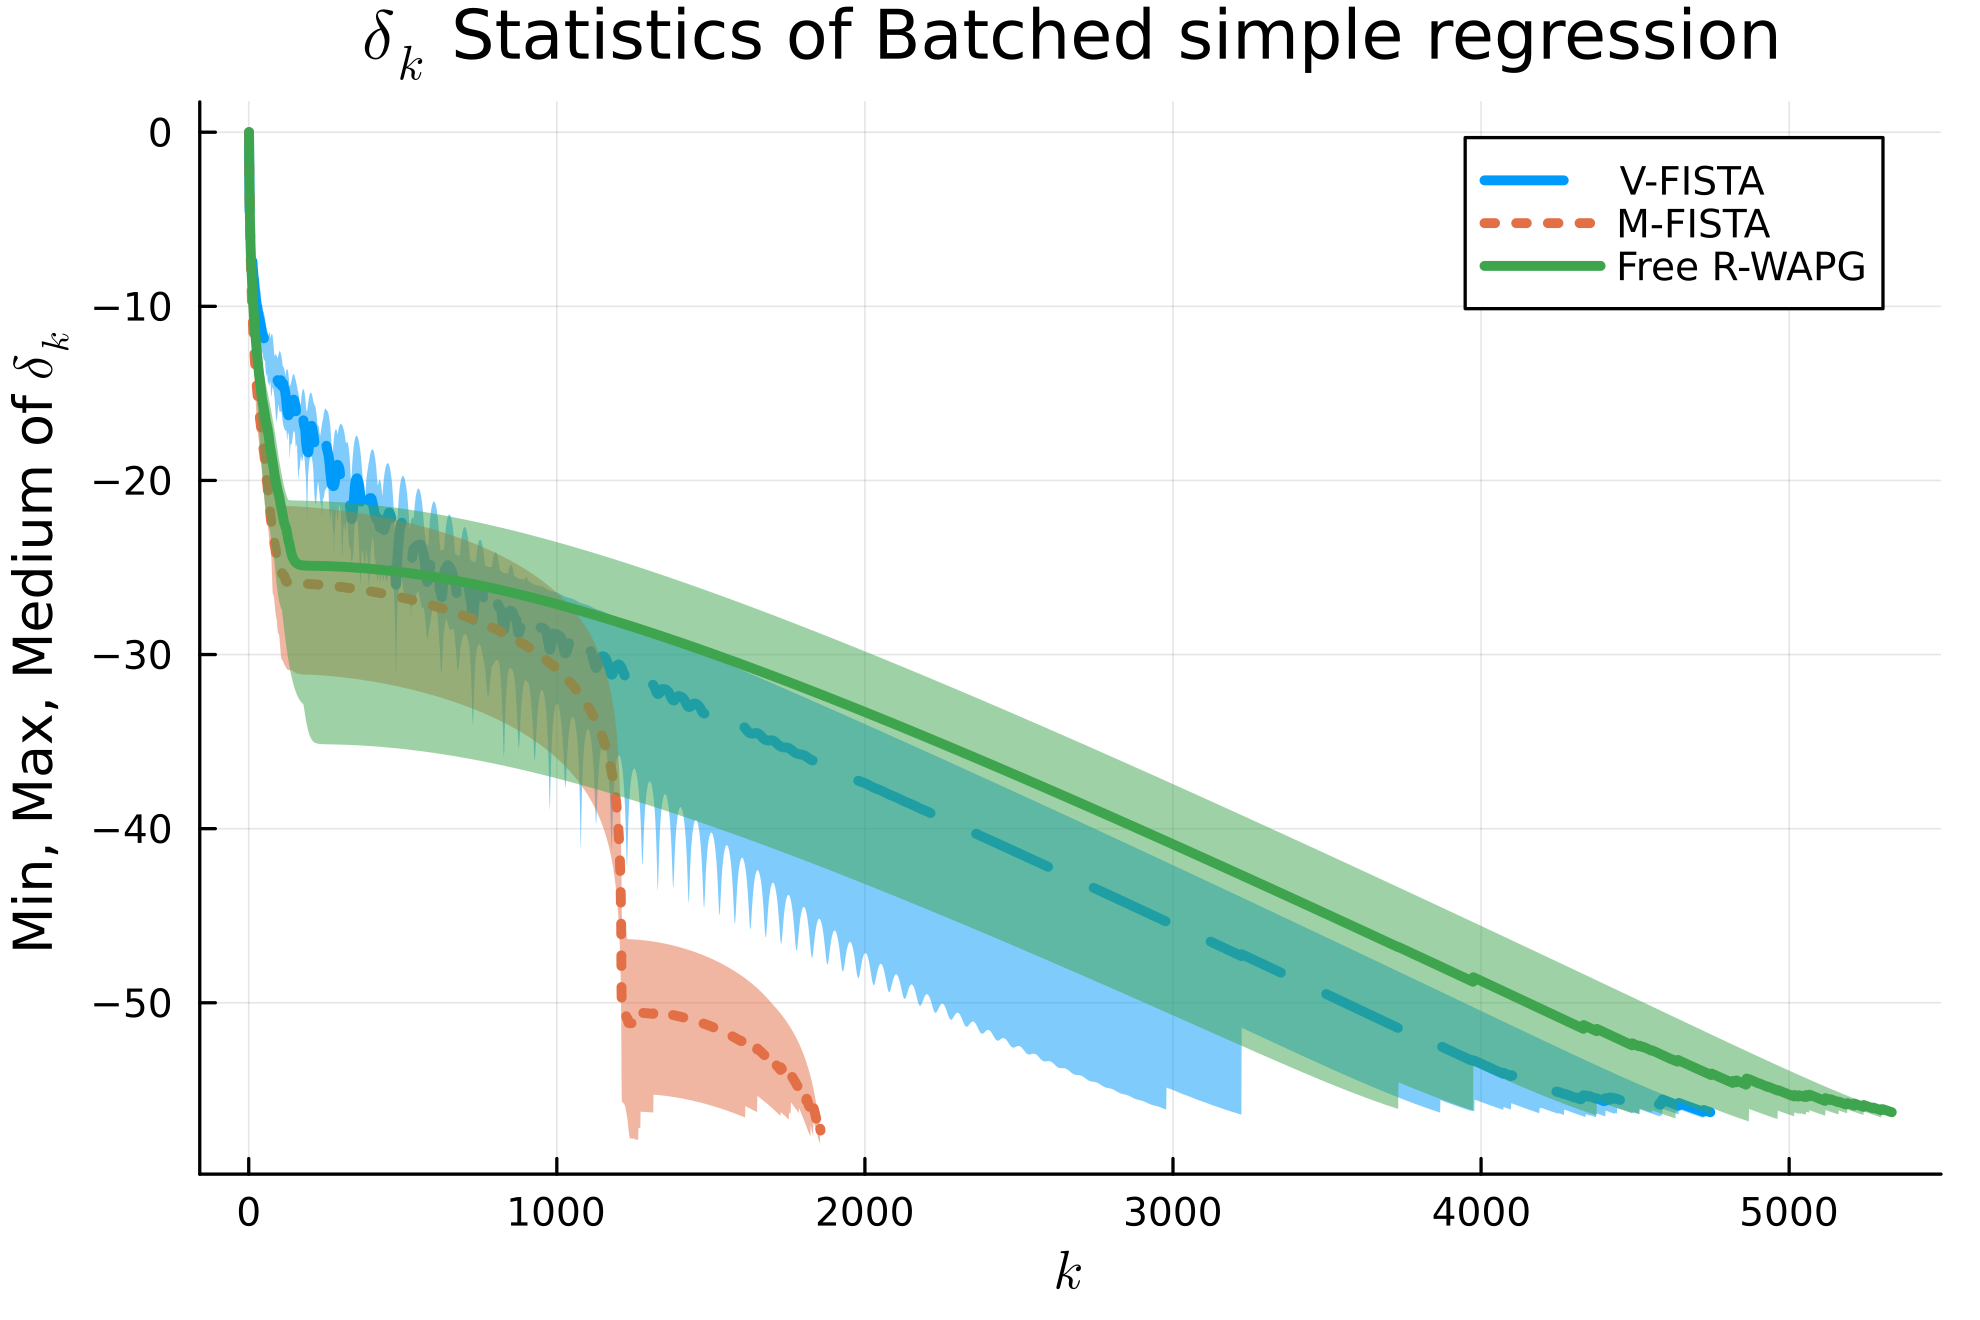
\includegraphics[width=\textwidth]{assets/simple_regression_batched-256.png}
                    \caption{$N = 256$, simple convex quadratic.}
                \end{subfigure}
                \hfill
                \begin{subfigure}[b]{0.47\textwidth}
                    \centering
                    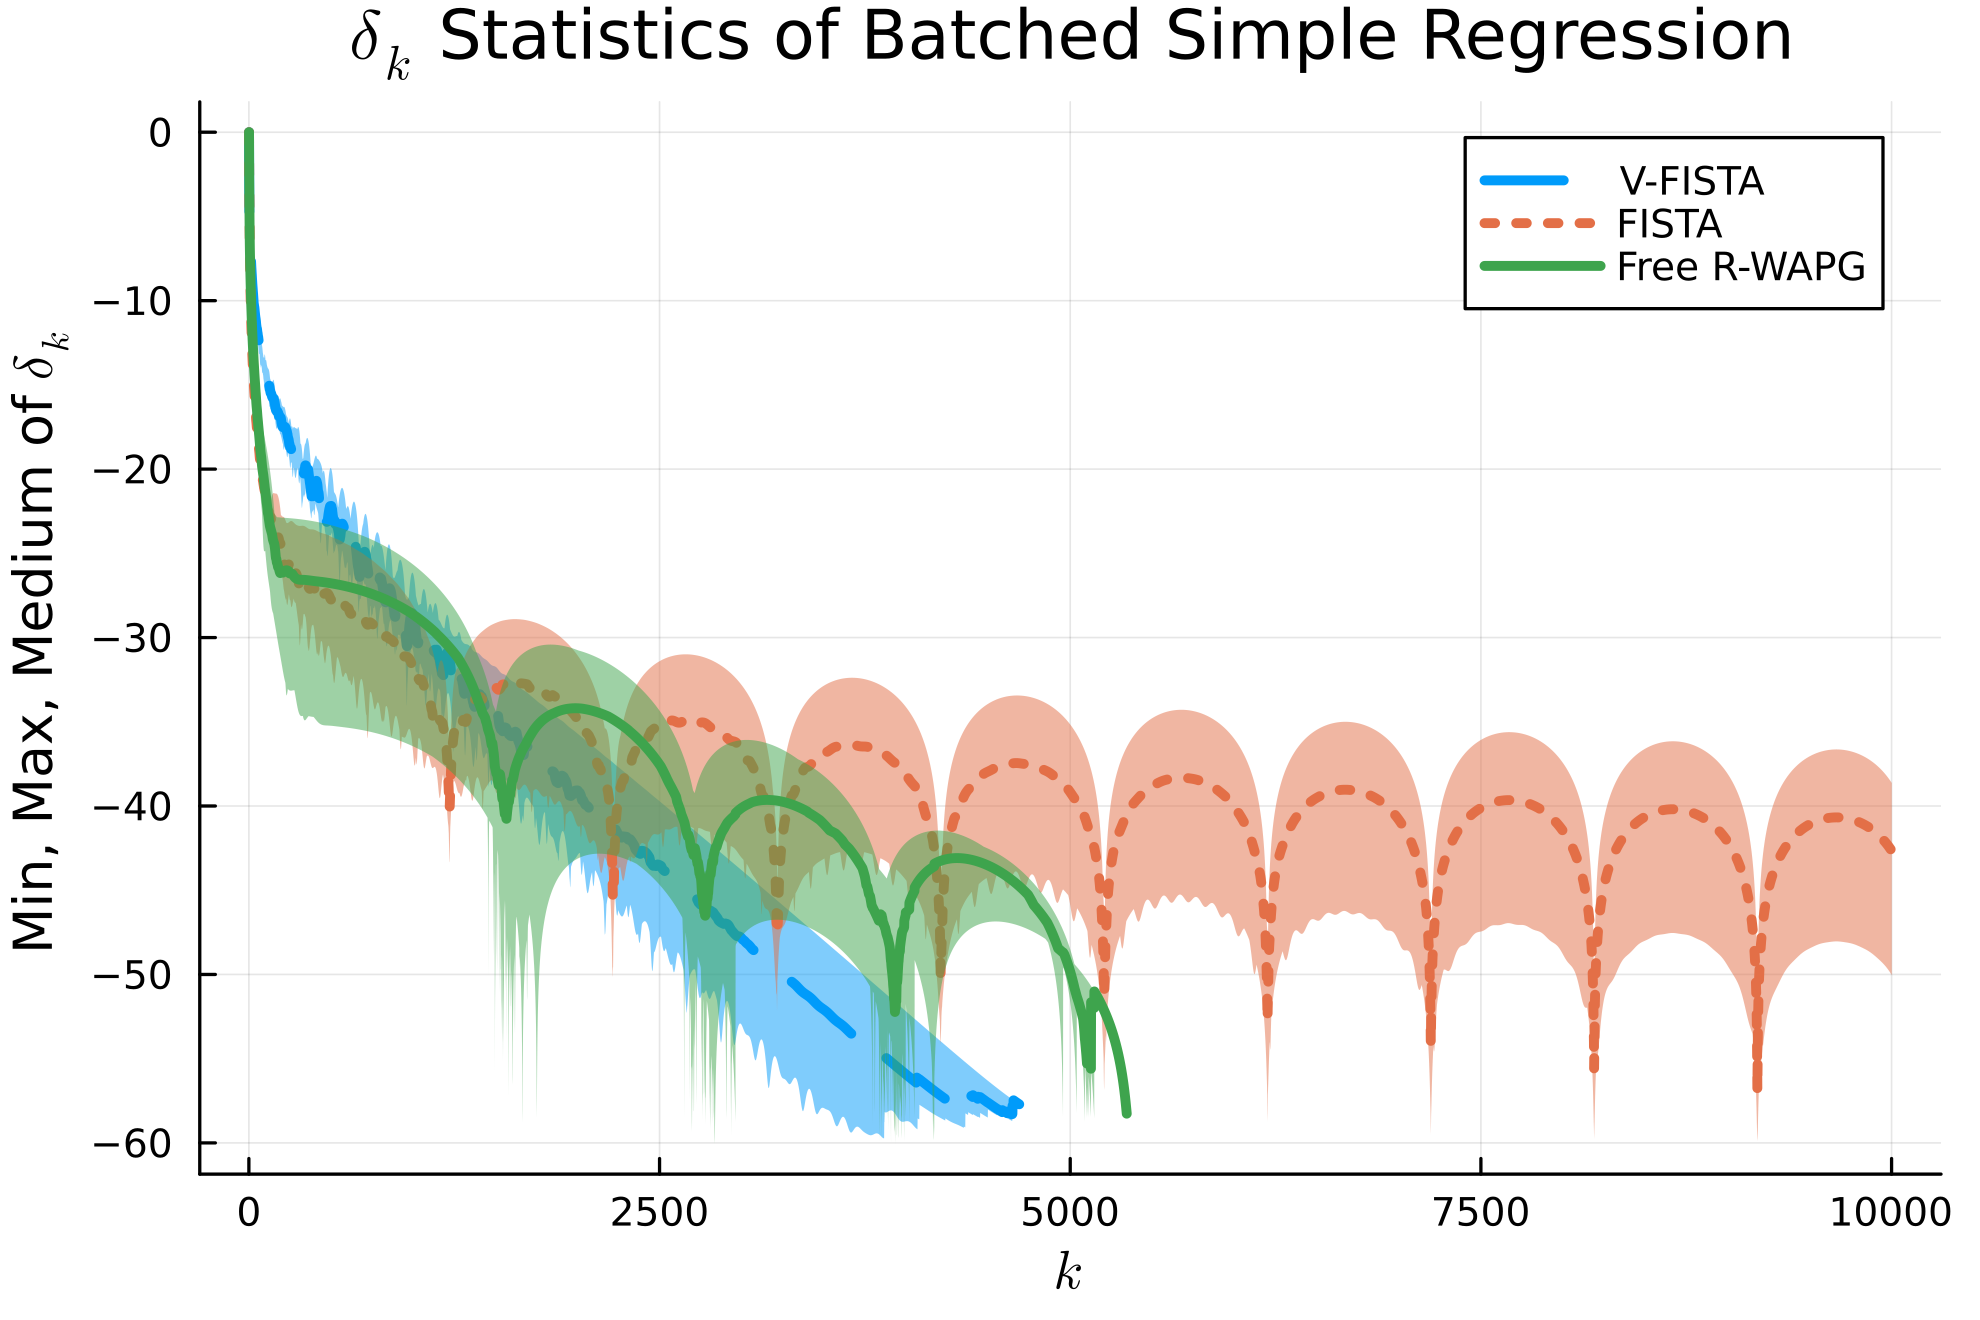
\includegraphics[width=\textwidth]{assets/simple_regression_batched-1024.png}
                    \caption{$N = 1024$, simple convex quadratic. }
                \end{subfigure}
                \caption{
                    Statistics for experiments with simple convex quadratic for V-FISTA, M-FISTA, and R-WAPG.
                }
                \label{fig:simple-quadratic-NOG}
            \end{figure}
        \end{frame}
        \begin{frame}{$\mu$ estimations}
            Free R-WAPG estimates $\mu_k$ each iteration. 
            The value of $\mu_k$ had been recorded for one trial and this is a plot of the estimations: 
            \begin{figure}[H]
                \centering
                \begin{subfigure}[b]{0.47\textwidth}
                    \centering
                    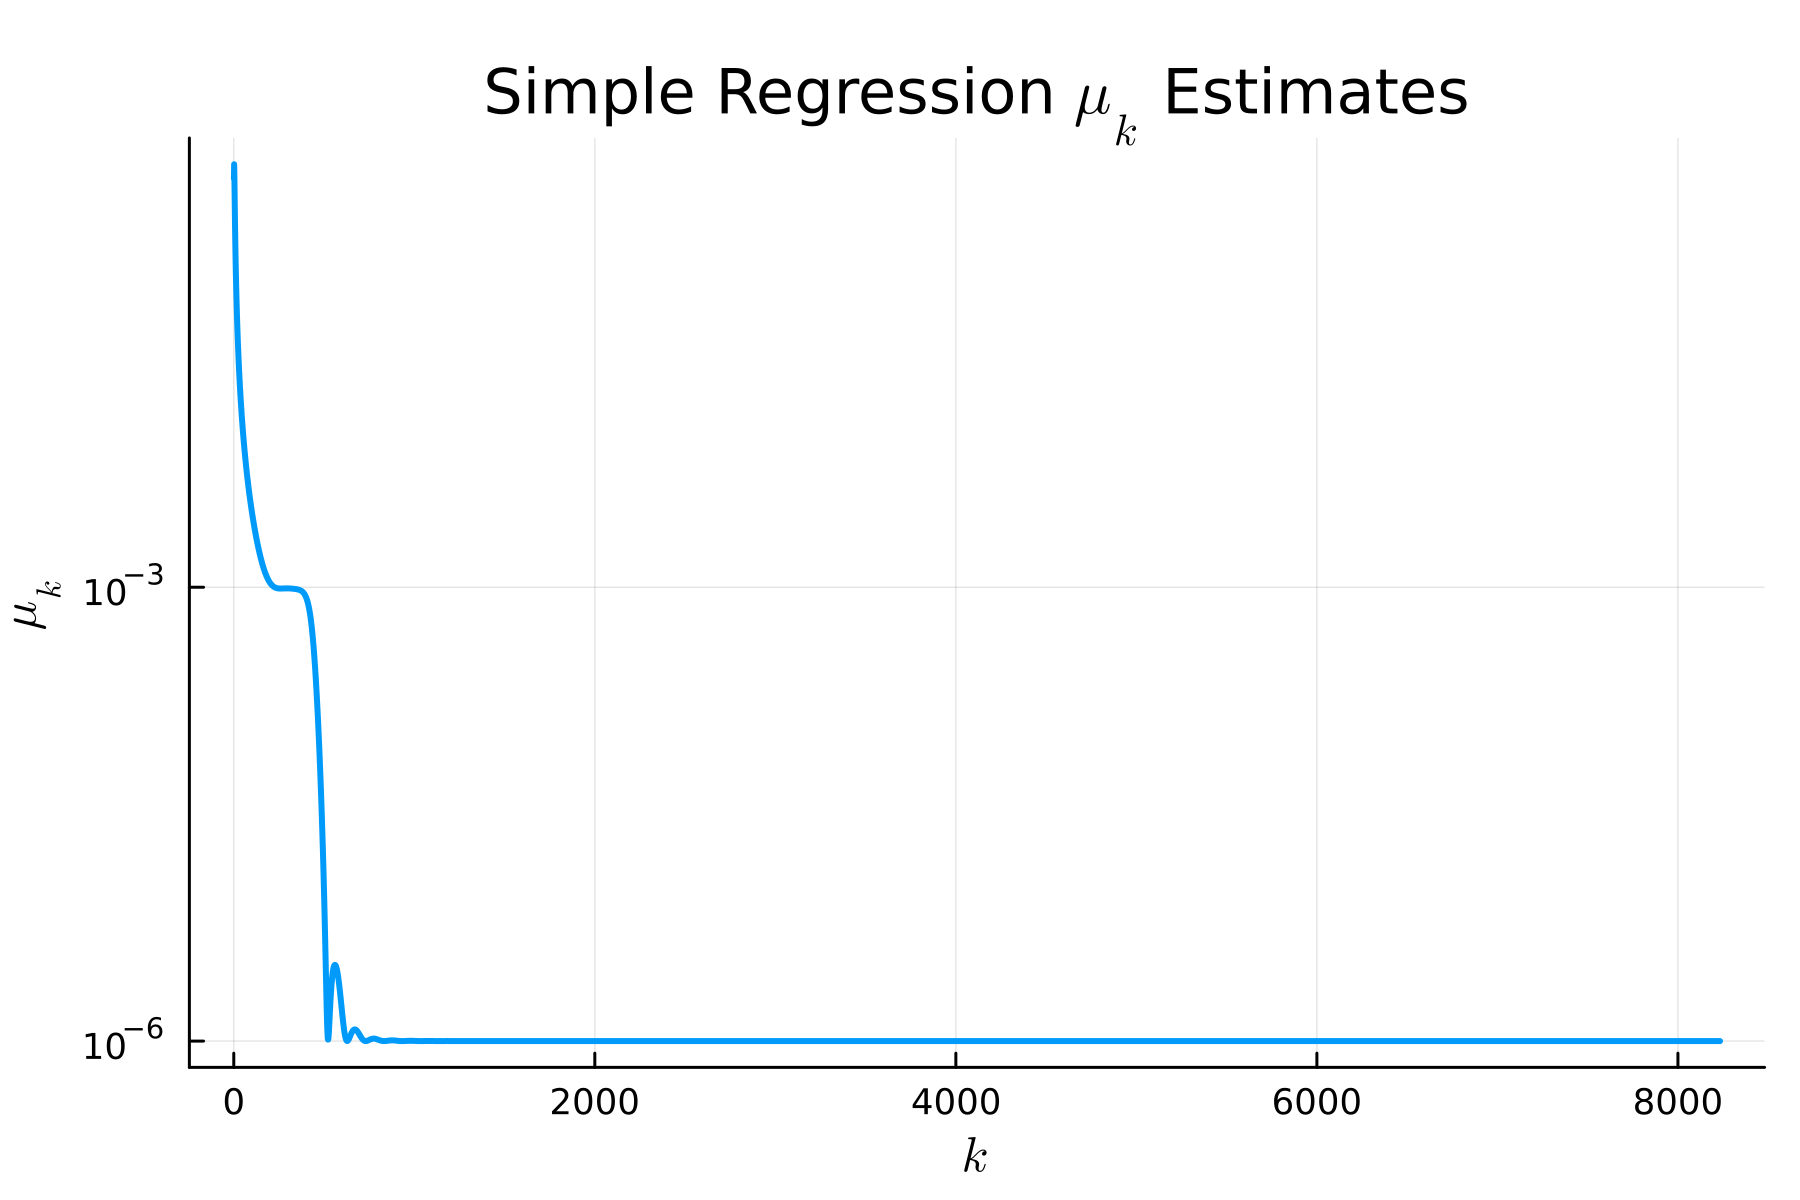
\includegraphics[width=\textwidth]{assets/simple_regression_loss_sc_estimates_1024.png}
                \end{subfigure}
                \hfill
                \begin{subfigure}[b]{0.47\textwidth}
                    \centering
                    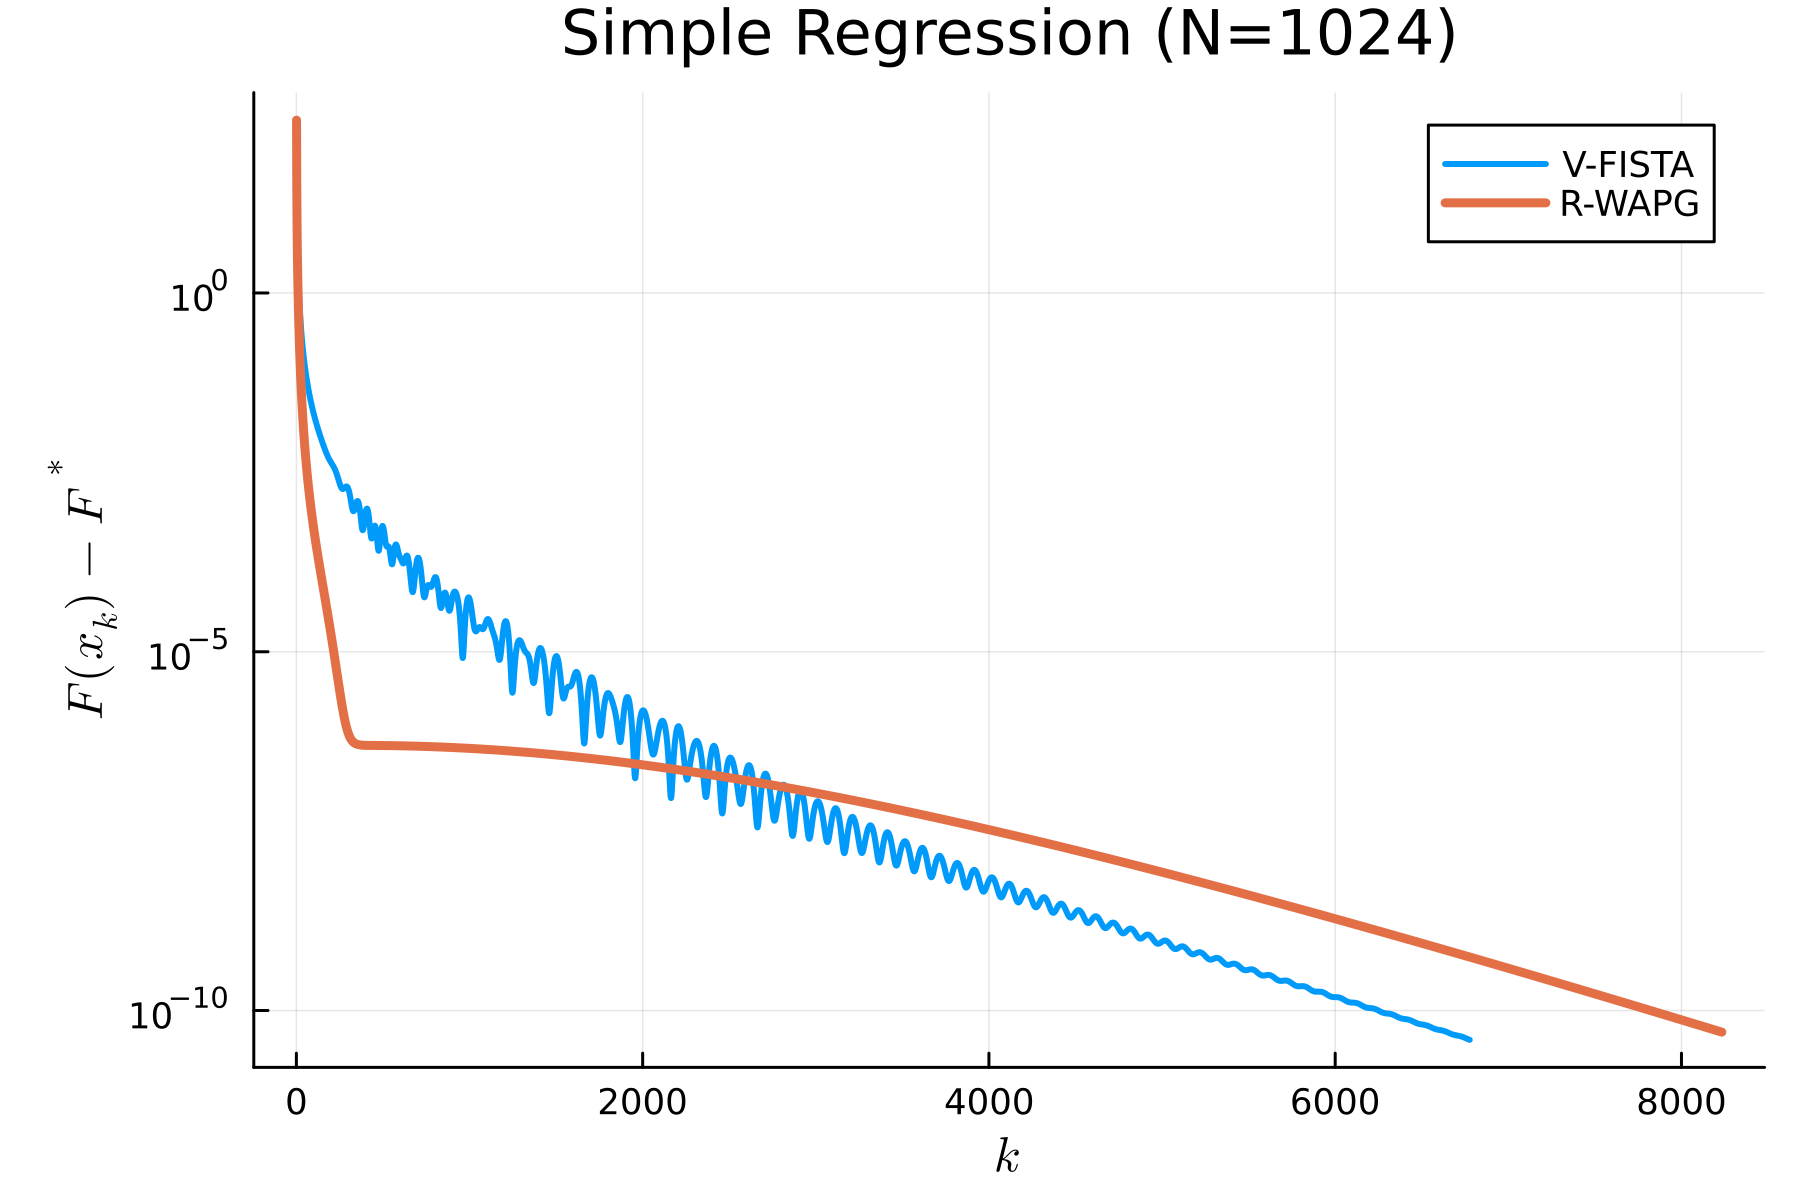
\includegraphics[width=\textwidth]{assets/simple_regression_loss_1024.png}
                \end{subfigure}
                \caption{
                    $N = 1024$, the $\mu$ estimates produced by Algorithm \ref{alg:free-rwapg} (R-WAPG) is recorded.
                }
                \label{fig:simple-quadratic-r-wapg-mu-estimates}
            \end{figure}
        \end{frame}
        \begin{frame}{Real time R-WAPG upper bound}
            By collecting $(\alpha_k)_{k \ge 0}$ while the algorithm is running we made the following plot for the simple quadratic experiment. 
            \begin{figure}[H]
                \centering
                \begin{subfigure}[b]{0.75\textwidth}
                    \centering
                    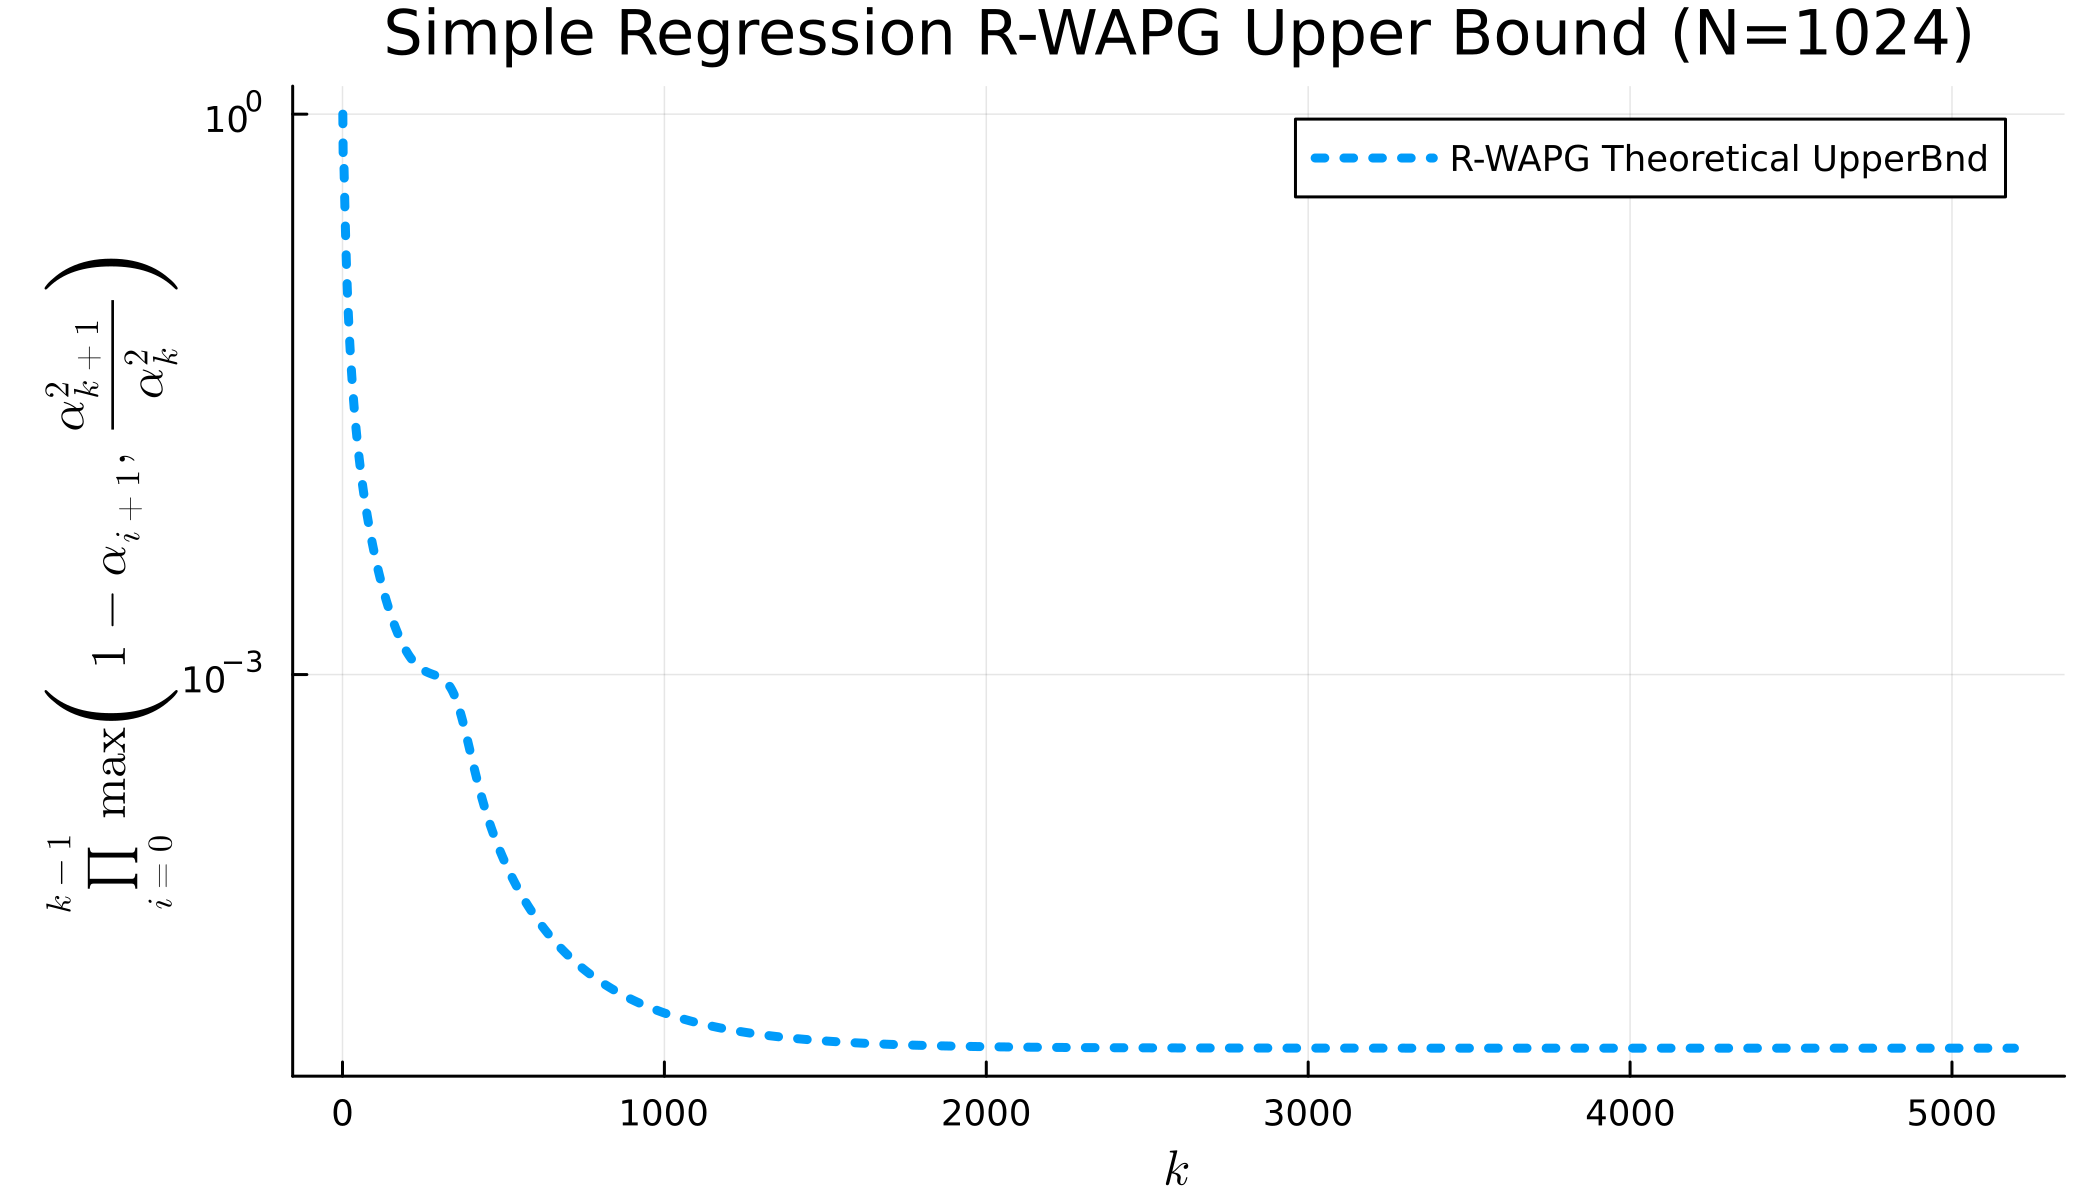
\includegraphics[width=\textwidth]{
                        assets/simple_regression_rwapg_upperbnd_1024.png
                    }
                \end{subfigure}
                \caption{
                    $N = 1024$, the upper bound estimates in real time from the collected $(\alpha_k)_{k \ge 0}$ sequence. 
                }
                \label{fig:simple-quadratic-r-wapg-rwapg-upperbnd}
            \end{figure}
        \end{frame} 
    \subsection{Numerical experiment, LASSO}
        \begin{frame}{The LASSO problem}
            The problem of LASSO from Tibshirani \cite{tibshirani_regression_1996} is the optimization problem $\min_{x \in \RR^n}\{(1/2)\Vert Ax - b\Vert^2 - \lambda\Vert x\Vert_1\}$. 
            \begin{enumerate}
                \item $A \in \RR^{N \times N}$, full of i.i.d random variable from a standard normal distribution. 
                \item Computed in prior, $L, \mu$ are parameters estimated by $\mu = 1/\Vert (A^TA)^{-1}\Vert$ and $L = \Vert A^TA\Vert$. The norm is the spectral norm. 
                \item The smallest value of $F(x_k)$, for all algorithms, over all tries are taken as an estimate of $F^+$. 
            \end{enumerate}
        \end{frame}
        \begin{frame}{Results plotted}
            With $A\in \RR^{N\times N}$ fixed, for each $x_0 \sim \mathcal N(I, \mathbf 0)$ realized, 30 experiments are preformed and the medium, minimum and maximum of $\delta_k$ are recorded for M-FISTA, Free R-WAPG, and V-FISTA. 
            \begin{figure}[H]
                \begin{subfigure}[b]{0.47\textwidth}
                    \centering
                    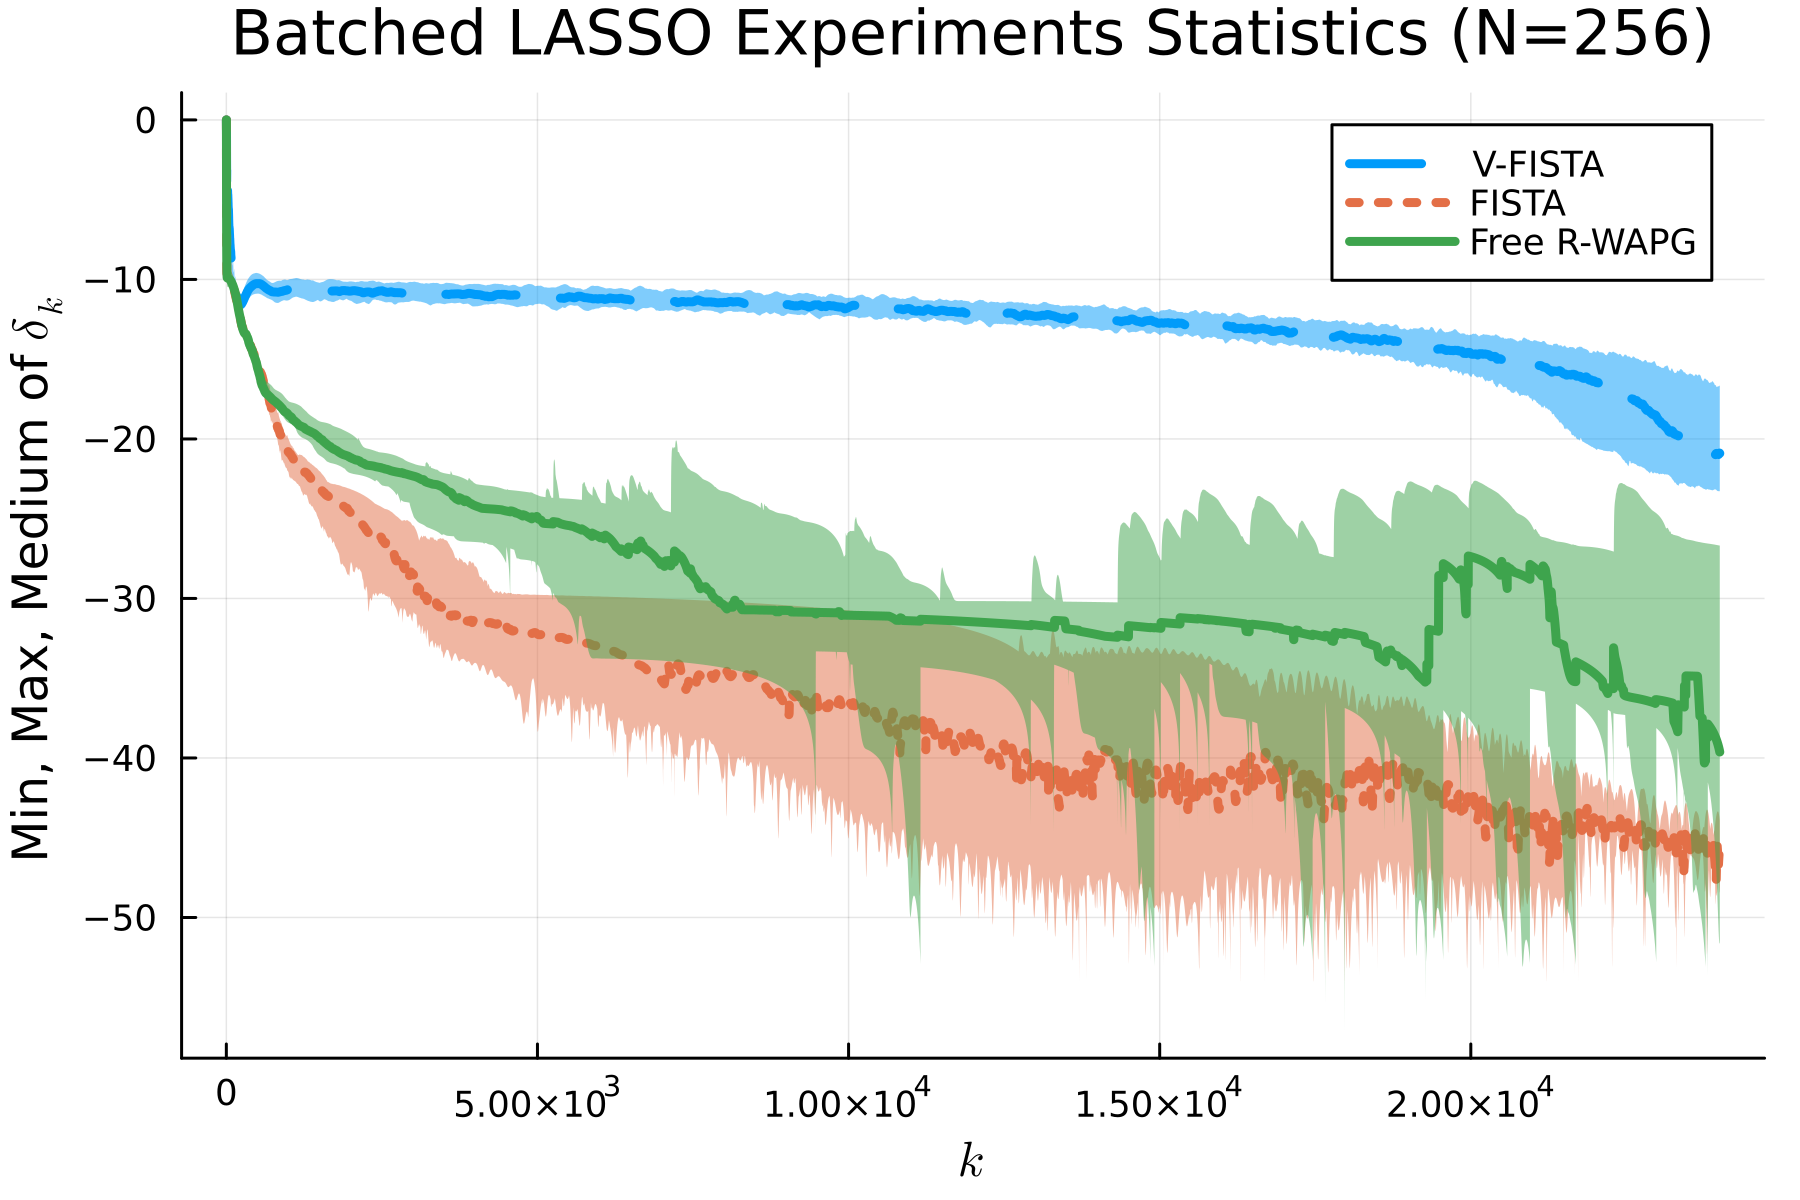
\includegraphics[width=\textwidth]{assets/lasso_batched_statistics_64-256.png}
                    \caption{LASSO experiment with $M = 64, N = 256$. Plots of minimum, maximum, and median $\delta_k$ with estimated $F^*$. }
                \end{subfigure}
                \begin{subfigure}[b]{0.47\textwidth}
                    \centering
                    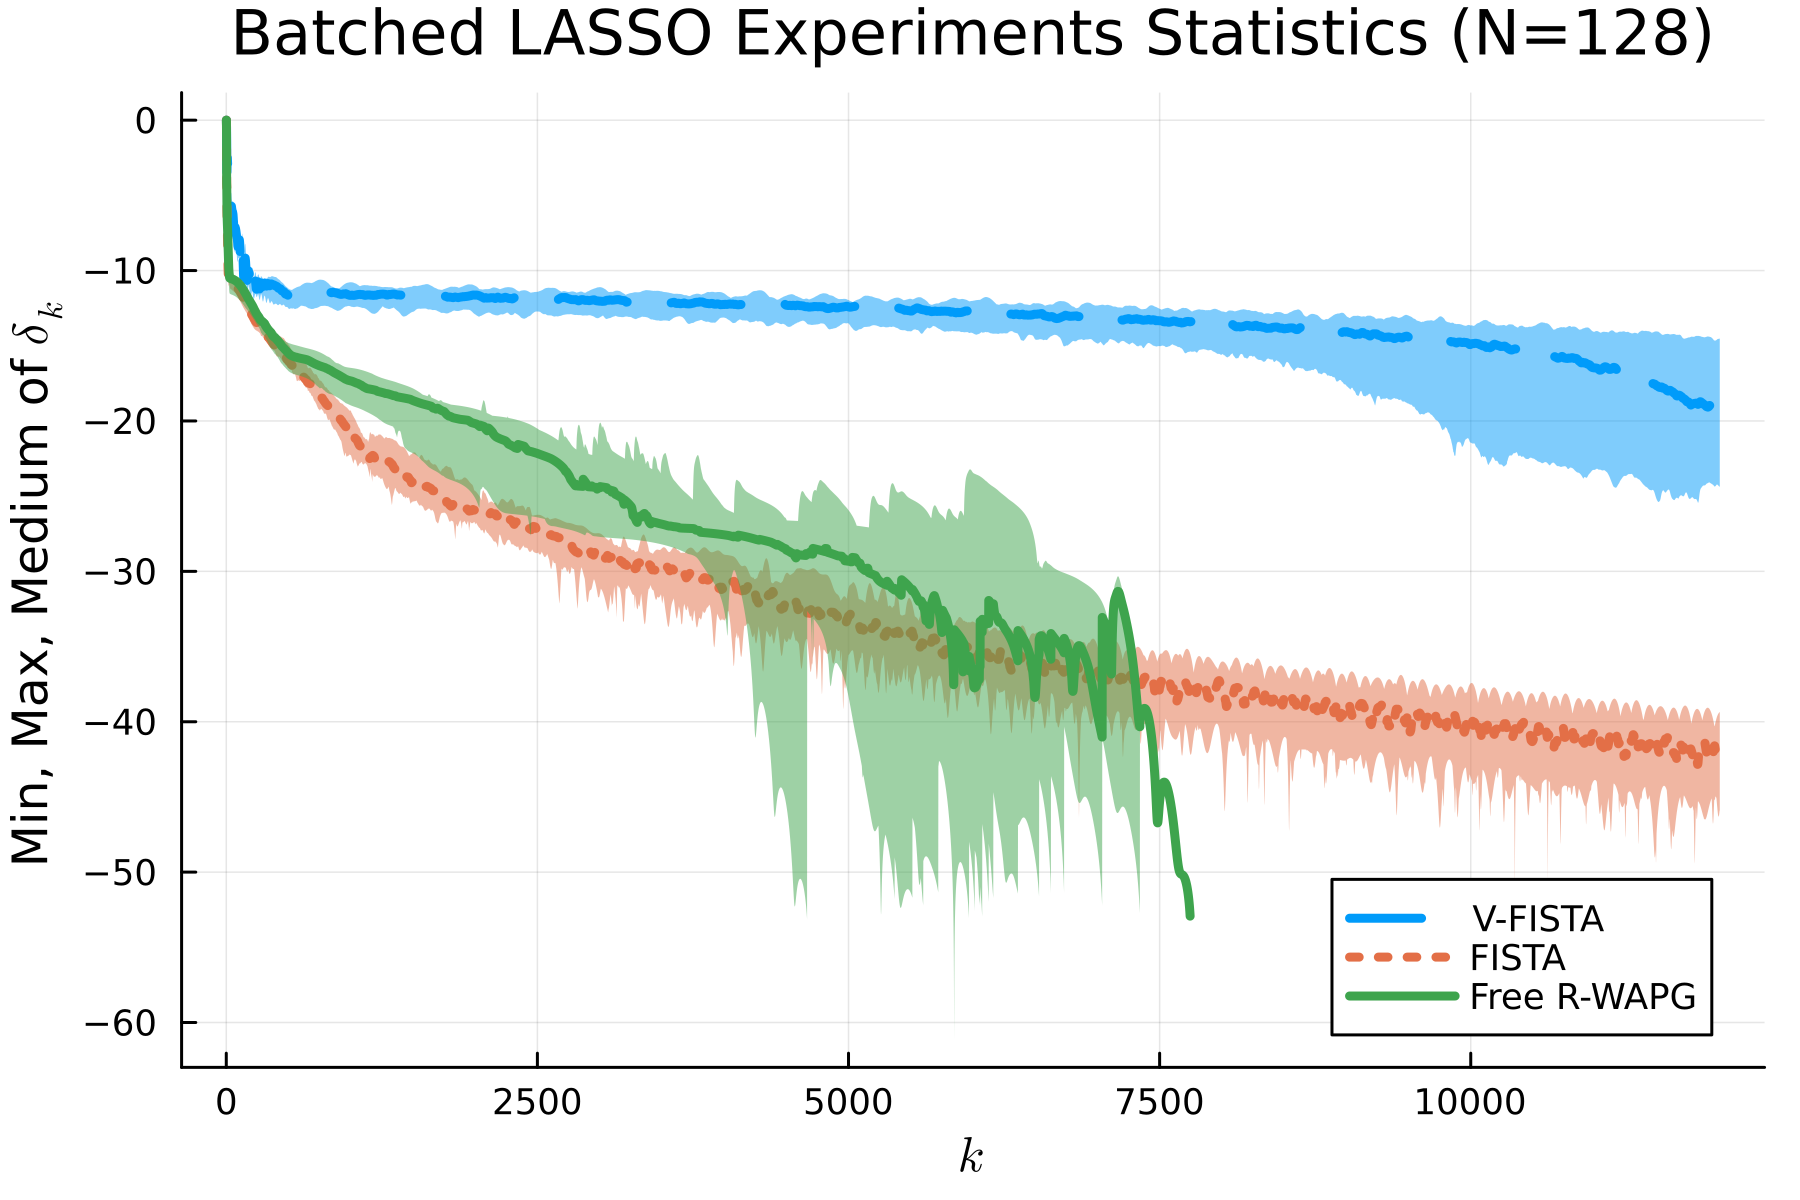
\includegraphics[width=\textwidth]{assets/lasso_batched_statistics_64-128.png}
                    \caption{LASSO experiment with $M = 64, N = 128$. Plots of minimum, maximum, and median $\delta_k$ with estimated $F^*$. }
                \end{subfigure}
                \caption{LASSO experiments statistics for test algorithms. }
                \label{fig:batched-lasso}
            \end{figure}
        \end{frame}
        \begin{frame}{Estimates of strong convexity constant}
            The parameters in this specific trial are $\mu = 7.432363627613958\times 10^{-18}$ and $L = 2321.737206983643$. 
            \begin{figure}[H]
                \begin{subfigure}[b]{0.47\textwidth}
                    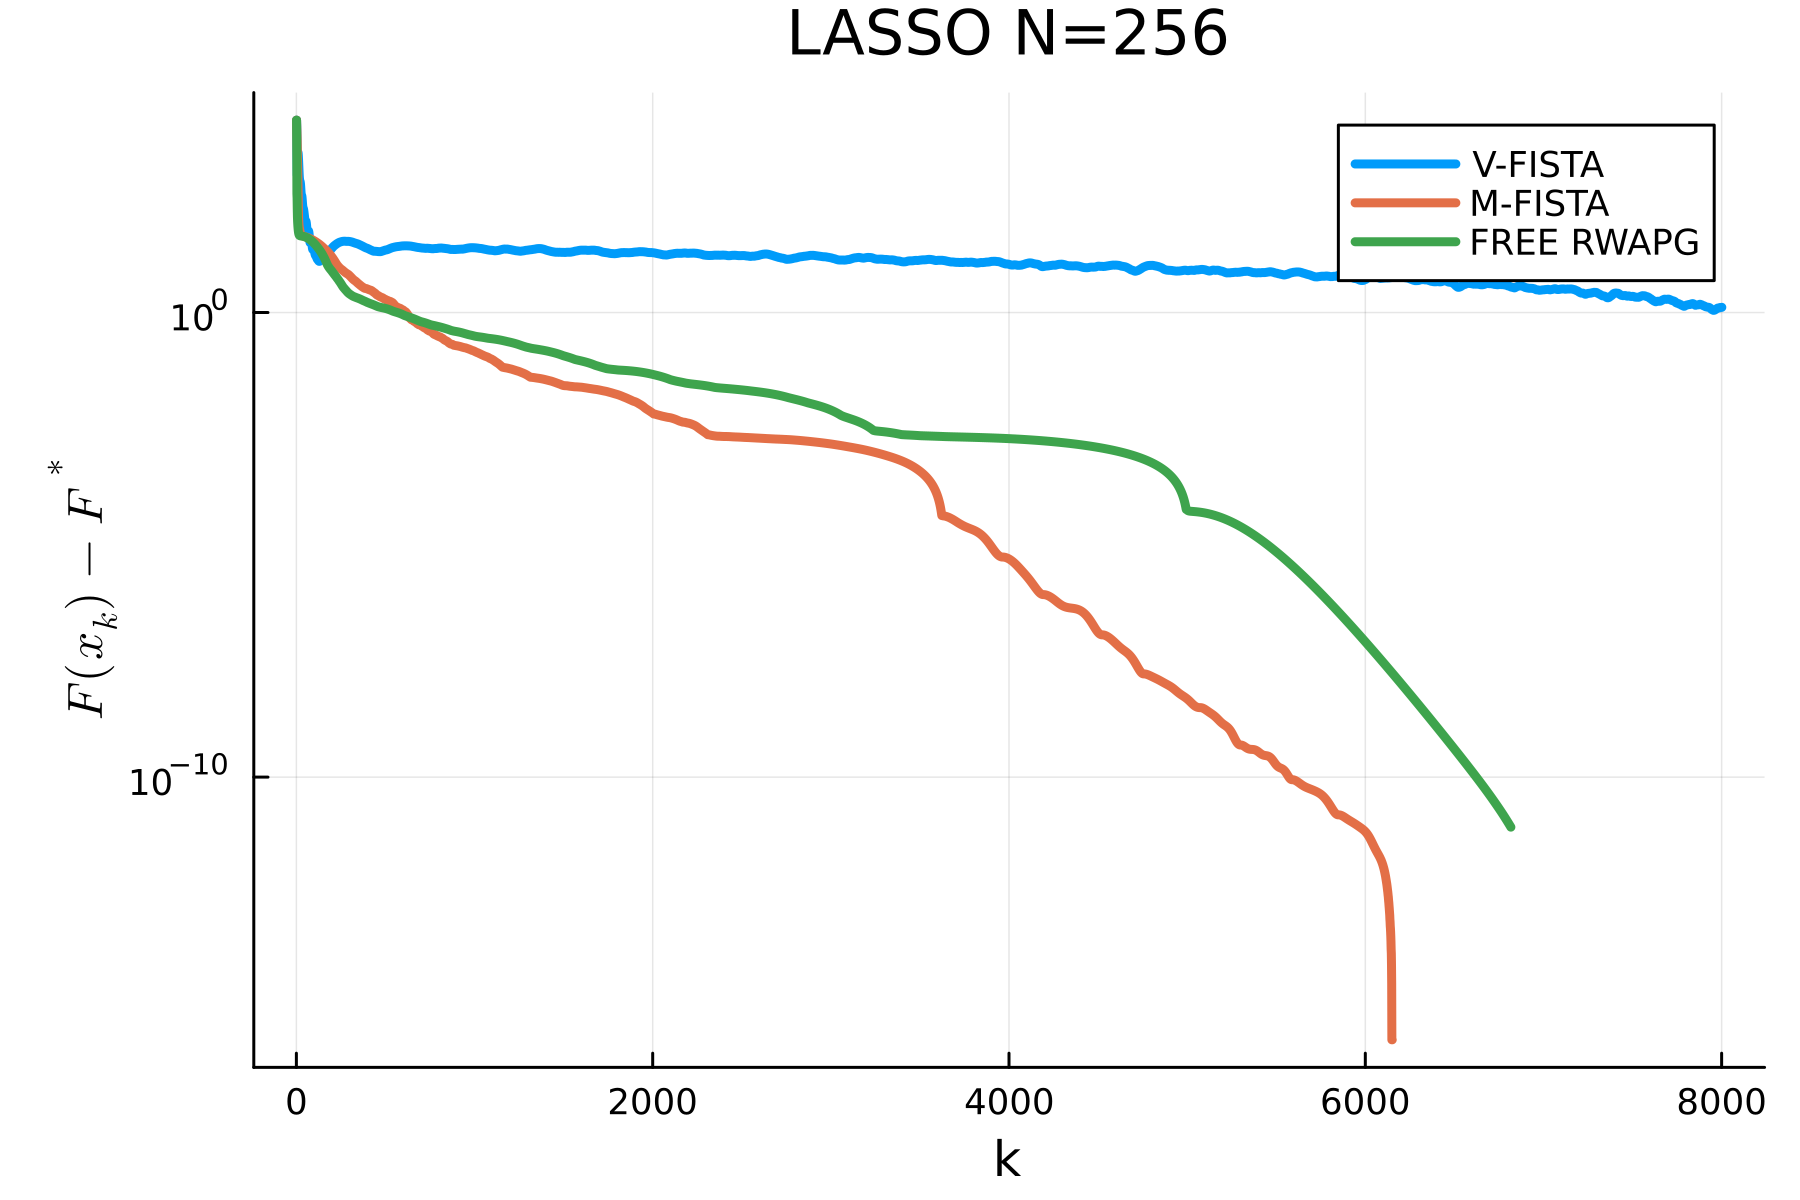
\includegraphics[width=\textwidth]{assets/lasso_loss_256.png}
                    \caption
                    {A single run of LASSO experiment displaying $F(x_k) - F^*$ for several test algorithms.
                    }
                \end{subfigure}
                \begin{subfigure}[b]{0.47\textwidth}
                    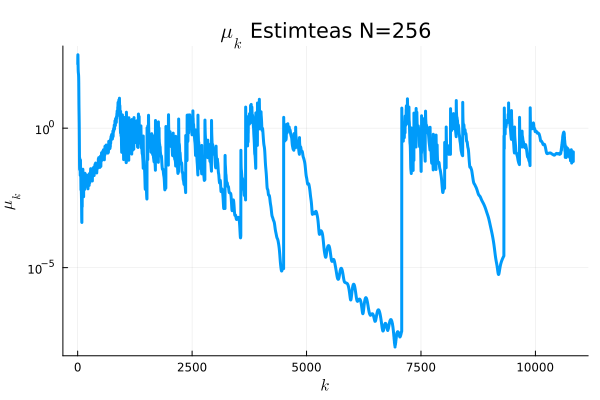
\includegraphics[width=\textwidth]{assets/lasso_sc_estimates_256.png}
                    \caption{The $\mu_k$ estimated by FR-WAPG for one LASSO experiment. }
                \end{subfigure}
                \caption{A single LASSO experiment results, with $M = 64, N=256$.}
                \label{fig:single-lass-mu-estimates}
            \end{figure}
        \end{frame}
        \begin{frame}{Real time R-WAPG upper bound}
            Below is the plot of the real time estimates of R-WAPG convergence bound using for the LASSO experiment. 
            \begin{figure}[H]
                \centering
                \begin{subfigure}[b]{0.75\textwidth}
                    \centering
                    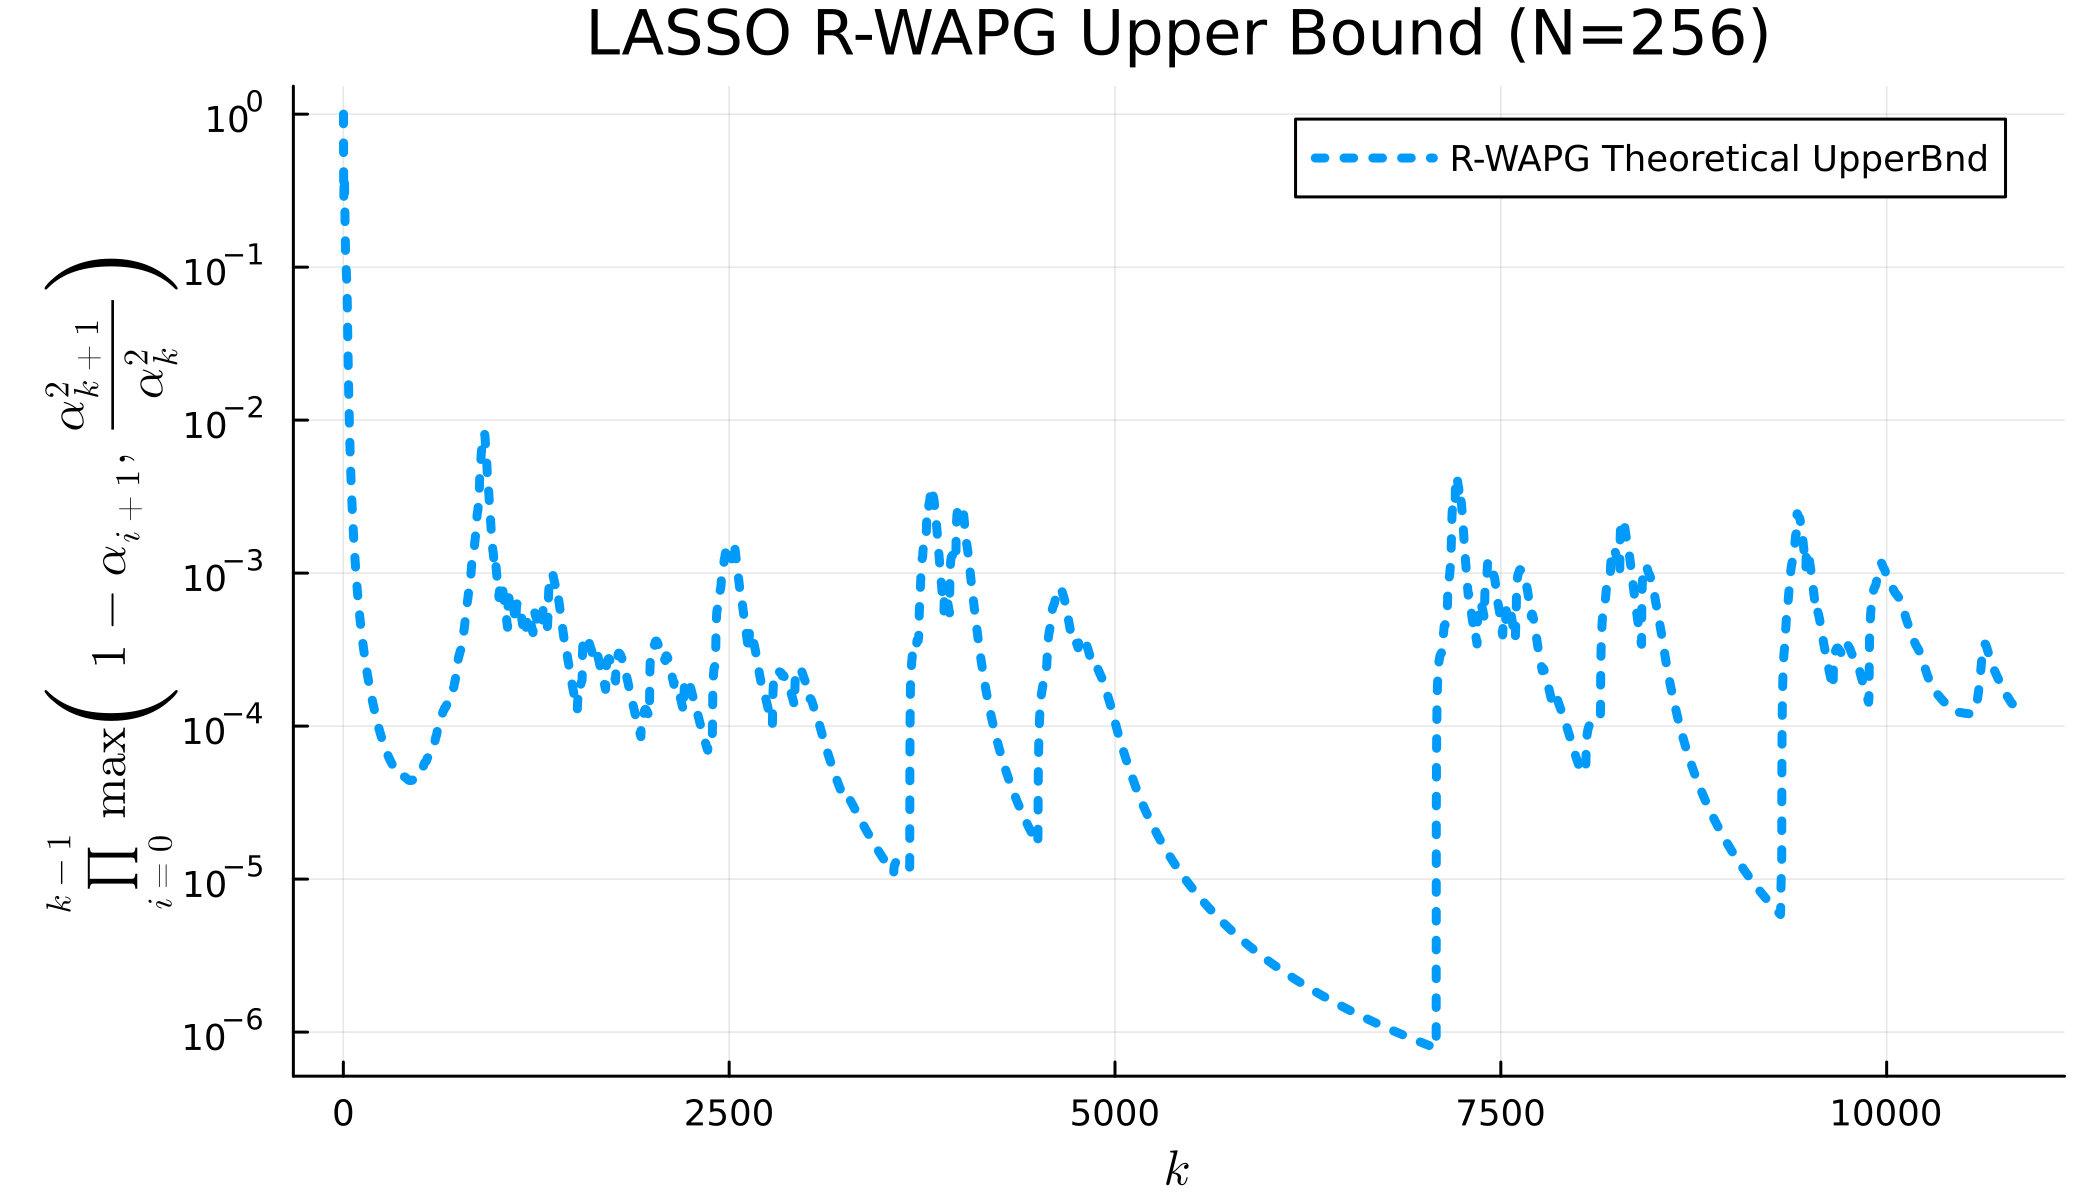
\includegraphics[width=\textwidth]{
                        assets/lasso_rwapg_upperbnd_256.png
                    }
                \end{subfigure}
                \caption{
                    $N = 1024$, the upper bound estimates in real time from the collected $(\alpha_k)_{k \ge 0}$ sequence. 
                }
                \label{fig:single-lass-r-wapg-rwapg-upperbnd}
            \end{figure}
        \end{frame}

\section{References and draft on arxiv}
    \begin{frame}{Thanks for the participations. Merci pour les participations.}
        Our paper can be found on arxiv using the following QR code: 
        \begin{figure}
            \centering
            
\includegraphics[width=15em]{assets/paper-qrcode.png}
        \end{figure}
        Questions?
    \end{frame}
    \begin{frame}{References}        
        \bibliography{references/R-WAPG.bib}
    \end{frame}

\end{document}